\chapter{概率生成模型}
\label{chap:pgm-generative}

生成模型既用于评价给定观测的概率，也用于生成新观测，这两项任务的计算代价可能相差很大。例如，从噪声到图像的网络可以迅速输出样本，而给定图像的密度可能难以求值；采用条件分解的模型可以精确评价完整观测的似然，生成时却可能需要逐个输出分量。图分解、边缘化和近似推断把这些差异落实为具体计算：先确定查询的概率对象，再找出其中未观测的变量，以及需要执行的求和、积分或变量变换。

本章考察三种构造复杂观测分布的机制：潜变量边缘化、可逆变量变换和人工随机过程。每种机制都需要说明分布为何归一化、训练目标如何联系似然，以及生成样本所需的计算。神经网络分别参数化条件分布、可逆映射或局部转移；这些概率角色决定了模型的表达限制、学习误差和查询成本。

\section{概率生成模型的共同问题}
\label{sec:pgm-generative-common}

设训练样本$\bm{x}_1,\ldots,\bm{x}_n$独立同分布地来自未知分布$p_{\mathrm{data}}$，用参数向量$\bm{\theta}$确定的$p_{\bm{\theta}}$近似数据分布。除特别说明外，观测取值于$\mathbb{R}^{d}$，本章用连续密度描述它们：区域上的概率由密度积分得到，单点密度值可以大于$1$。二值或离散观测则用概率质量函数描述，各个取值的质量直接表示其概率。比较模型似然时，各模型需采用相同的观测表示和测度。

\term{概率生成模型}（probabilistic generative model）为可能出现的观测规定一个分布，并据此生成新观测。对显式密度模型，归一化要求$\int p_{\bm{\theta}}(\bm{x})\,\mathrm{d}\bm{x}=1$。最大似然学习最小化
\begin{equation}
  \label{eq:pgm-generative-nll}
  J(\bm{\theta})
  =-\frac{1}{n}\sum_{i=1}^{n}\log p_{\bm{\theta}}(\bm{x}_i).
\end{equation}
计算该目标需要评价每个观测的对数密度。潜变量模型中的积分可能成为主要障碍；只给出噪声到观测的生成程序时，还需要确认观测密度是否存在，以及如何求值。因此，模型的训练规则、密度评价、采样步骤和潜变量推断各有独立的计算要求。

自回归模型用归一化的一维条件分布按链式法则构成联合分布。给定完整观测后，各条件分布可以直接评价；祖先采样则通常按照分解顺序生成各分量（见第~\ref{sec:pgm-static-directed-autoregressive}节）。以此为基线，下面考察三种计算安排：VAE通过潜变量积分定义观测密度，规范化流用双射的体积变化追踪密度，扩散模型通过多次局部随机转移生成观测。

三种机制使用的概率结构有所不同。VAE采用有向潜变量图；离散扩散采用沿人工噪声索引展开的有向Markov链；规范化流依靠确定性双射和变量变换公式，其计算图记录变换依赖，条件独立性仍需由相应概率模型确定。后文还将介绍概率电路：它通过约束计算图的结构支持精确边缘化和条件查询，补充上述三种机制在查询方面的取舍。

本章用一维目标$X\sim\mathcal{N}(0,5)$贯穿三种机制。独立高斯变量相加、标准高斯缩放和以该分布为起点的前向扩散，分别提供可解析的例子。相同的观测分布使比较集中于潜变量含义、密度计算和随机路径，而复杂数据的表达限制将在各机制中另行讨论。

\section{变分自编码器}
\label{sec:pgm-generative-vae}

\subsection{有向潜变量模型}
\label{sec:pgm-generative-latent-model}

潜变量模型用未观测因素解释观测中共同变化的部分：先抽取潜变量，再按给定潜变量的条件分布生成观测。\term{变分自编码器}（variational autoencoder, VAE）为这一生成模型配备可学习的近似后验。生成网络参数化条件分布，推断网络根据观测给出潜变量的近似分布；两者通过变分目标共同训练\scite{kingma2013}

令$\bm{z}\in\mathbb{R}^{k}$，通常取先验$p(\bm{z})=\mathcal{N}(\bm{0},\bm{I}_k)$，再用神经网络输出条件分布$p_{\bm{\theta}}(\bm{x}\mid\bm{z})$的参数。生成联合分布与观测边缘分布为
\begin{equation}
  \label{eq:pgm-generative-vae-joint}
  \begin{aligned}
    p_{\bm{\theta}}(\bm{x},\bm{z})
      &=p(\bm{z})p_{\bm{\theta}}(\bm{x}\mid\bm{z}),\\
    p_{\bm{\theta}}(\bm{x})
      &=\int p(\bm{z})p_{\bm{\theta}}(\bm{x}\mid\bm{z})
          \,\mathrm{d}\bm{z}.
  \end{aligned}
\end{equation}
先验和每个条件分布归一化时，交换非负积分的次序即可证明观测分布归一化。评价某个观测的似然仍需要计算式中的潜变量积分，其难度取决于条件分布的形式和潜变量维数。

对于连续观测，\term{解码器}（decoder）输出给定潜变量时观测分布的参数。常用的各向同性高斯设定为
\begin{equation}
  \label{eq:pgm-generative-gaussian-decoder}
  p_{\bm{\theta}}(\bm{x}\mid\bm{z})
  =\mathcal{N}\bigl(\bm{x};
    \bm{g}_{\bm{\theta}}(\bm{z}),\tau^2\bm{I}_d\bigr),
  \qquad \tau>0.
\end{equation}
其中$\bm{g}_{\bm{\theta}}:\mathbb{R}^{k}\to\mathbb{R}^{d}$给出条件均值，$\tau^2$为条件噪声方差。一次完整生成先抽取$\bm{z}\sim p$，再抽取独立标准高斯噪声$\bm{\eta}$，得到$\bm{x}=\bm{g}_{\bm{\theta}}(\bm{z})+\tau\bm{\eta}$。实际展示也可能只输出条件均值$\bm{g}_{\bm{\theta}}(\bm{z})$；这会省去观测噪声，与式~\eqref{eq:pgm-generative-gaussian-decoder}规定的随机采样对应不同输出。

线性解码器$\bm{g}_{\bm{\theta}}(\bm{z})=\bm{W}\bm{z}+\bm{b}$与独立高斯噪声共同构成线性高斯模型，其中$\bm{W}\in\mathbb{R}^{d\times k}$。将潜变量变换的协方差与噪声协方差相加，得到观测边缘分布（见第~\ref{sec:pgm-static-directed-linear-gaussian}节）：
\[
  p_{\bm{\theta}}(\bm{x})
  =\mathcal{N}\bigl(\bm{x};
    \bm{b},\bm{W}\bm{W}^{\top}+\tau^2\bm{I}_d\bigr).
\]

潜变量后验可以通过配平方求得。对数联合分布中，先验和观测似然的二次项相加，给出后验精度矩阵$\bm{I}_k+\tau^{-2}\bm{W}^{\top}\bm{W}$；线性项进一步确定后验均值：
\begin{equation}
  \label{eq:pgm-generative-linear-posterior}
  \begin{aligned}
    \bm{\Sigma}
      &=\bigl(\bm{I}_k+\tau^{-2}\bm{W}^{\top}\bm{W}\bigr)^{-1},\\
    \bm{m}(\bm{x})
      &=\tau^{-2}\bm{\Sigma}\bm{W}^{\top}(\bm{x}-\bm{b}),\\
    p_{\bm{\theta}}(\bm{z}\mid\bm{x})
      &=\mathcal{N}\bigl(\bm{z};\bm{m}(\bm{x}),\bm{\Sigma}\bigr).
  \end{aligned}
\end{equation}

非线性解码器可以表达弯曲、非高斯的观测分布。此时，$\lVert\bm{x}-\bm{g}_{\bm{\theta}}(\bm{z})\rVert_2^2$通常不再是潜变量的二次式，前述配平方计算便失去适用条件，边缘密度和后验一般需要近似求解。VAE保留式~\eqref{eq:pgm-generative-vae-joint}的生成定义，用近似后验支持参数学习。

\begin{example}[同一观测分布的潜变量解释]
  \label{ex:pgm-generative-gaussian-latent}
  取$Z\sim\mathcal{N}(0,1)$、$E\sim\mathcal{N}(0,1)$且二者独立，令$X=2Z+E$，于是$X\sim\mathcal{N}(0,5)$。观测$x=2$后，
  \[
    p(z\mid x=2)\propto
    \exp\left[-\frac{1}{2}\{z^2+(2-2z)^2\}\right]
    \propto\exp\left[-\frac{5}{2}(z-0.8)^2\right].
  \]
  后验为$\mathcal{N}(0.8,0.2)$。独立观测噪声使多个潜变量取值都可以解释$x=2$，因此给定观测后仍保留潜变量不确定性。后文的Flow则为完整观测规定唯一逆像。
\end{example}

\subsection{VAE目标与摊销后验}
\label{sec:pgm-generative-vae-objective}

观测边缘积分难以求值时，可以用近似后验构造证据下界。将式~\eqref{eq:pgm-generative-vae-joint}的联合分解代入一般ELBO，得到条件对数似然的期望减去后验与先验的KL散度（见式~\eqref{eq:pgm-variational-elbo}）：
\begin{equation}
  \label{eq:pgm-generative-vae-elbo}
  \begin{aligned}
    \mathcal{L}(\bm{\theta},\bm{\phi};\bm{x})
    ={}&\mathbb{E}_{q_{\bm{\phi}}(\bm{z}\mid\bm{x})}
       [\log p_{\bm{\theta}}(\bm{x}\mid\bm{z})]\\
      &-\operatorname{KL}\bigl(
       q_{\bm{\phi}}(\bm{z}\mid\bm{x})\,\|\,p(\bm{z})\bigr)
      \leq\log p_{\bm{\theta}}(\bm{x}).
  \end{aligned}
\end{equation}

\term{编码器}（encoder）根据观测输出$q_{\bm{\phi}}(\bm{z}\mid\bm{x})$的分布参数。同一组权重$\bm{\phi}$在不同观测之间共享，均值和尺度随输入变化；这构成摊销推断，$\bm{\phi}$对应第~\ref{sec:pgm-variational-amortized}节的$\bm{\omega}$。生成参数$\bm{\theta}$属于观测条件分布。图~\ref{fig:pgm-generative-vae}分别表示两套计算：先验与解码器规定生成联合分布，编码器在训练和观测后推断时提供近似后验。

\begin{figure}[htbp]
  \centering
  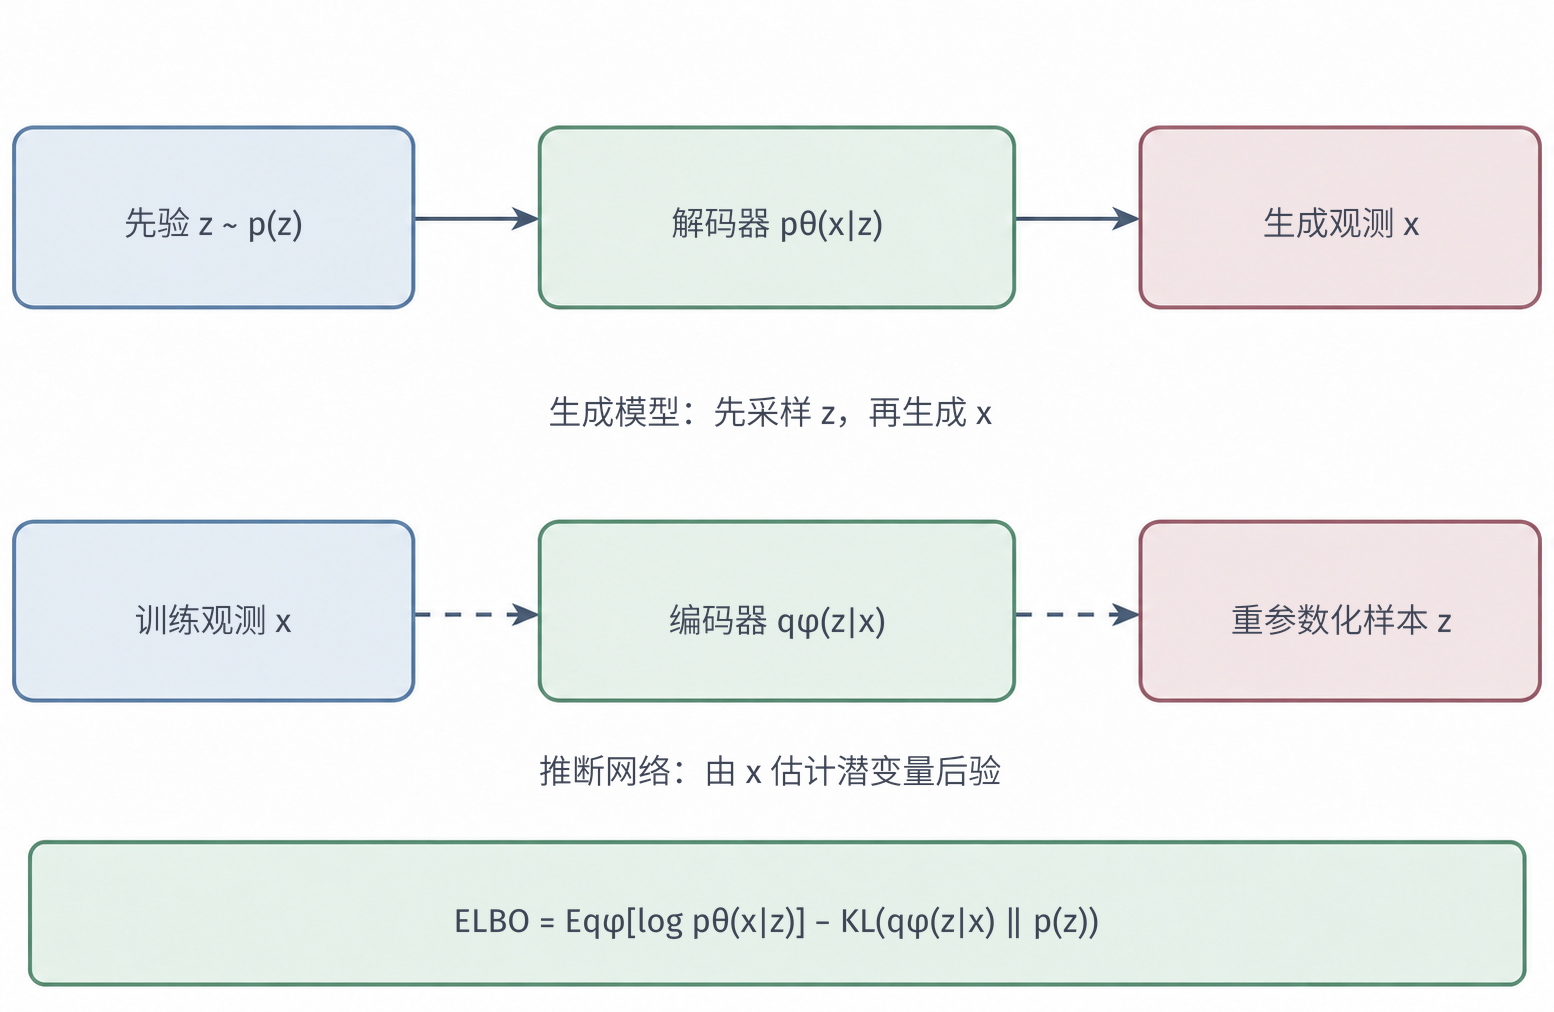
\includegraphics[width=112.000mm]{figures/03-models/03-probabilistic-graphical-models/generated/pgm-generative-vae/figure.png}
  \caption{VAE的生成与近似推断。上行实线表示从先验抽潜变量，再按$p_{\bm\theta}(\bm x\mid\bm z)$抽观测；下行虚线表示由观测构造$q_{\bm\phi}(\bm z\mid\bm x)$。两行分别记录生成分布和推断程序，底部ELBO联系条件似然与近似后验。}
  \label{fig:pgm-generative-vae}
\end{figure}

常用编码器取对角高斯
\[
  q_{\bm{\phi}}(\bm{z}\mid\bm{x})
  =\mathcal{N}\!\left(
    \bm{z};\bm{m}_{\bm{\phi}}(\bm{x}),
    \operatorname{diag}\bigl(\bm{s}_{\bm{\phi}}^2(\bm{x})\bigr)
    \right),
\]
其中每个$s_{\bm{\phi},j}(\bm{x})>0$。网络可以输出对数方差，再经指数变换得到正方差。对标准高斯先验，KL项解析可得：
\begin{equation}
  \label{eq:pgm-generative-diagonal-kl}
  \operatorname{KL}(q_{\bm{\phi}}\,\|\,p)
  =\frac{1}{2}\sum_{j=1}^{k}
     \bigl(m_{\bm{\phi},j}^2+s_{\bm{\phi},j}^2
            -1-\log s_{\bm{\phi},j}^2\bigr).
\end{equation}

式中省略了各分量对观测的依赖。为估计重构期望，抽取独立标准高斯噪声$\bm{\epsilon}$，经$\bm{z}=\bm{m}_{\bm{\phi}}(\bm{x})+\bm{s}_{\bm{\phi}}(\bm{x})\odot\bm{\epsilon}$得到后验样本，其中$\odot$表示逐元素乘法。噪声分布与网络参数无关，梯度可沿均值、尺度和解码器组成的可微路径计算（见第~\ref{chap:pgm-variational}章）。一次编码器前向计算给出当前观测的近似后验参数，省去了逐样本优化变分参数的步骤。

图~\ref{fig:vae-reparameterization-training}表示重参数化后的训练路径：独立噪声经编码器给出的均值与尺度变换为潜变量，重构项的梯度再通过解码器传回编码器。无条件生成采用先验样本进入解码器。

\begin{figure*}[htbp]
  \centering
  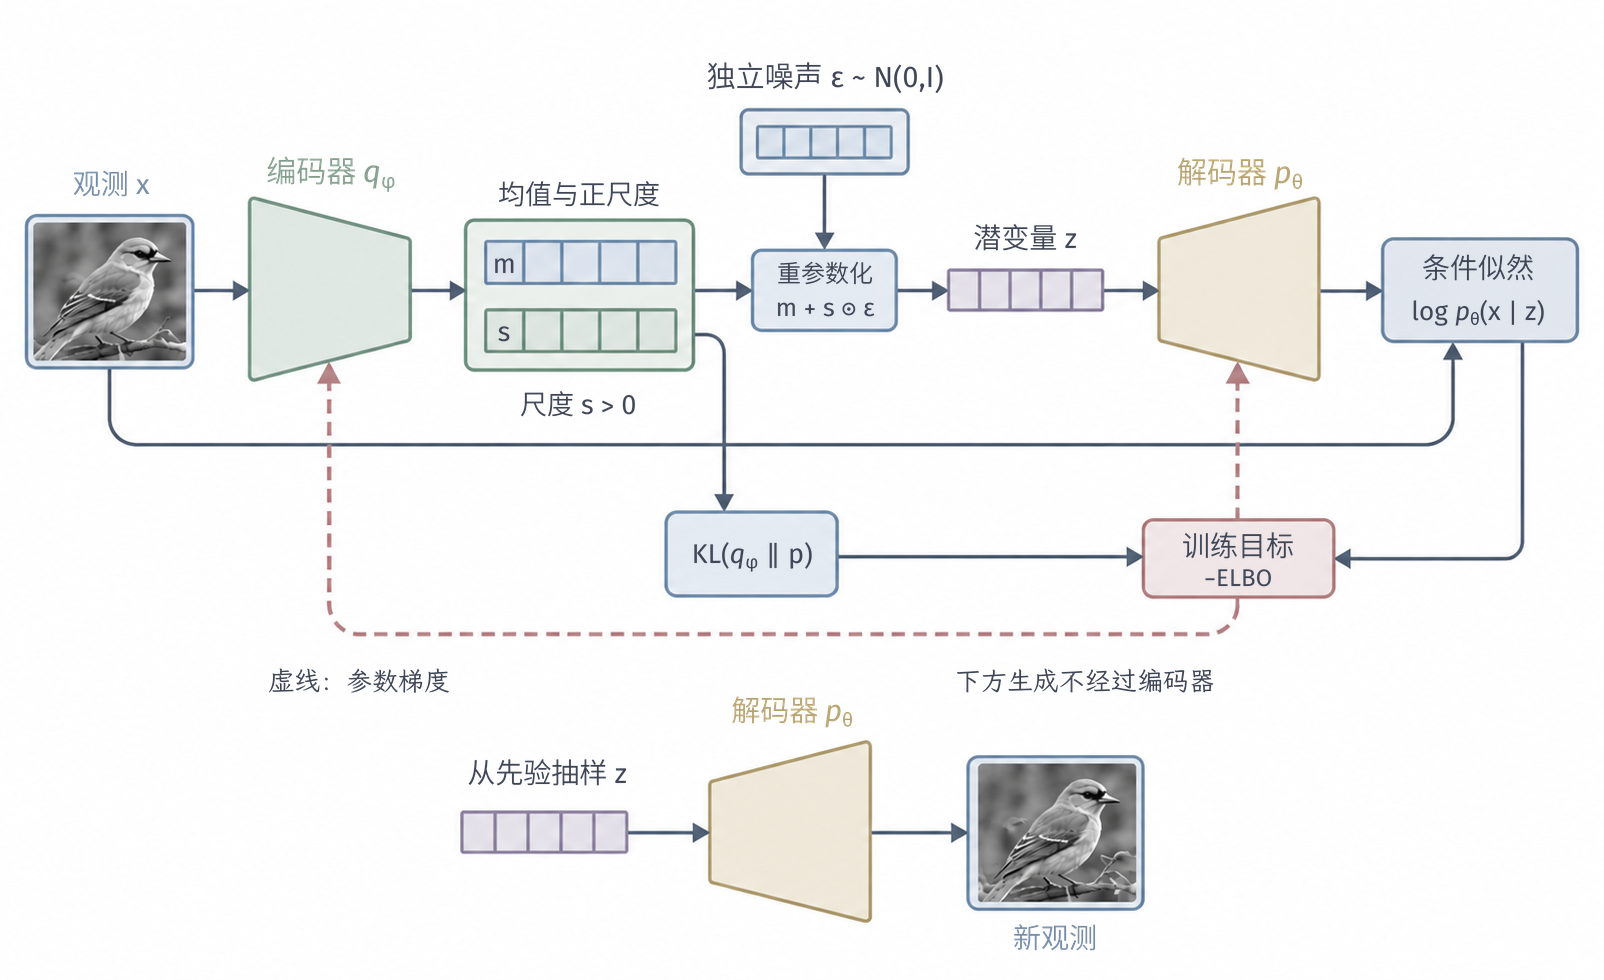
\includegraphics[width=135.805mm]{figures/03-models/03-probabilistic-graphical-models/generated/vae-reparameterization-training/figure.png}
  \caption{对角高斯VAE的重参数化与训练。编码器给出均值$\bm m$和正尺度$\bm s$，独立标准正态噪声经$\bm z=\bm m+\bm s\odot\bm\epsilon$形成潜变量，并进入解码器规定的条件分布。重构对数似然的期望与KL项组成ELBO，图中的负ELBO框表示训练目标。生成阶段从先验抽样，不经过编码器；鸟图为概念插画。}
  \label{fig:vae-reparameterization-training}
\end{figure*}

ELBO中的重构项由观测条件分布确定。对于式~\eqref{eq:pgm-generative-gaussian-decoder}的高斯解码器，负对数似然分解为加权平方误差和方差相关项：
\begin{equation}
  \label{eq:pgm-generative-reconstruction}
  -\log p_{\bm{\theta}}(\bm{x}\mid\bm{z})
  =\frac{\lVert\bm{x}-\bm{g}_{\bm{\theta}}(\bm{z})\rVert_2^2}
          {2\tau^2}
    +\frac{d}{2}\log(2\pi\tau^2).
\end{equation}
固定$\tau$时，最后一项与待学习参数无关。若方差参与学习，对数方差项与平方误差权重共同约束它：增大方差会减轻平方误差的代价，同时提高对数方差代价。删去后一项会改变优化目标。对于二值观测$x_j\in\{0,1\}$，采用给定潜变量后独立的Bernoulli分布，解码器输出参数$\pi_j(\bm{z})$，负对数似然为
\[
  -\sum_{j=1}^{d}
    \bigl[x_j\log\pi_j(\bm{z})
      +(1-x_j)\log(1-\pi_j(\bm{z}))\bigr].
\]

二值交叉熵由此来自Bernoulli观测假设。连续灰度值具有不同的取值空间；对它使用相同表达式时，需说明作为代理损失的含义。离散像素可以采用类别质量函数，也可以将连续条件密度在相应量化区间内积分得到概率质量。

在例~\ref{ex:pgm-generative-gaussian-latent}中，让编码器恰好输出$q(z\mid2)=\mathcal{N}(0.8,0.2)$，可以逐项复核ELBO：
\[
  \begin{aligned}
    \mathbb{E}_{q}(2-2Z)^2&=(2-1.6)^2+4(0.2)=0.96,\\
    \mathbb{E}_{q}\log p(2\mid Z)&=-\tfrac12\log(2\pi)-0.48,\\
    \operatorname{KL}(q\,\|\,p)&=
       \tfrac12\bigl(0.8^2+0.2-1-\log0.2\bigr).
  \end{aligned}
\]
各项相加得到$\mathcal{L}\approx-2.12366$，等于观测对数密度：
\[
  \log\mathcal{N}(2;0,5)
  =-\tfrac12\log(10\pi)-0.4.
\]
将近似后验改为先验时，ELBO降为$-\tfrac12\log(2\pi)-4\approx-4.91894$。两次计算使用相同生成模型，下界差异由近似后验与真实后验的匹配程度引起。

训练时，对小批量观测运行编码器，抽取标准噪声并计算ELBO的随机估计，再更新生成参数和共享编码器参数。停止条件可由计算预算或验证指标确定。设一次编码和解码的代价分别为$C_{\mathrm{enc}}$和$C_{\mathrm{dec}}$；每个观测使用一个潜变量样本时，前向代价约为$O(C_{\mathrm{enc}}+C_{\mathrm{dec}}+k)$，反向传播通常为同阶。增加后验样本可降低部分蒙特卡洛方差，同时增加解码计算。无条件生成只需先验采样和解码；观测后的近似推断只需一次编码器计算。

VAE的误差来自生成分布、近似后验和共享编码器三个层次。\term{模型近似误差}（model approximation error）由候选$p_{\bm{\theta}}$与数据分布的差距产生，需通过调整生成族处理。固定生成参数后，近似后验族的形状限制产生\term{近似族误差}（variational approximation error）。逐个观测的最优变分参数若无法由同一编码器同时表示，还会产生\term{摊销误差}（amortization error）。设$\mathcal{Q}$为候选后验族，$\mathcal{L}_{\mathcal{Q}}^*(\bm{x})=\sup_{q\in\mathcal{Q}}\mathcal{L}(\bm{\theta},q;\bm{x})$为固定模型下该族的最优下界，且$q_{\bm{\phi}}(\cdot\mid\bm{x})\in\mathcal{Q}$。下界差距可分解为
\begin{equation}
  \label{eq:pgm-generative-inference-gaps}
  \begin{aligned}
    \log p_{\bm{\theta}}(\bm{x})
      -\mathcal{L}(\bm{\theta},\bm{\phi};\bm{x})
    ={}&\bigl[\log p_{\bm{\theta}}(\bm{x})
             -\mathcal{L}_{\mathcal{Q}}^*(\bm{x})\bigr]\\
       &+\bigl[\mathcal{L}_{\mathcal{Q}}^*(\bm{x})
             -\mathcal{L}(\bm{\theta},\bm{\phi};\bm{x})\bigr].
  \end{aligned}
\end{equation}

第一项为近似族误差，第二项为当前编码器相对于逐观测最优解的差距，两项均非负。第二项还包含编码器优化不足；进一步比较最优共享编码器，可以区分摊销限制与优化误差（见式~\eqref{eq:pgm-variational-amortization-gap}）。增加生成族容量、扩大后验族和改进编码器优化，分别针对这些不同来源的误差。

\subsection{生成能力与失效模式}
\label{sec:pgm-generative-vae-failure}

潜变量维度决定生成模型可以用多少自由度解释观测变化。即使$k<d$，式~\eqref{eq:pgm-generative-gaussian-decoder}中正方差噪声仍覆盖全部观测维度，使模型具有$d$维密度。去掉噪声后，光滑低维解码器的输出通常集中于低维集合。增大潜变量维度可减轻表示瓶颈，同时增加学习和推断的自由度；这些维度能否承载有效信息，还取决于训练目标与解码器对潜变量的利用。

给定潜变量后若仍存在多种不同观测，固定方差的单一高斯条件似然通过平方误差拟合它们的均值。在有限二阶矩条件下，逐坐标的总体最优预测为$\mathbb E[\bm X\mid\bm z]$（参见\BookTheoremRef{thm:probability-conditional-mean-l2-projection}{第一卷“数学准备”的条件均值平方损失最优性定理}）。例如，边缘等概率出现在左右两处时，均值图像会在两处留下较淡的边缘，这提供了模糊重构的一种解释。表达力更强的条件似然可以分别描述这些结果；在简单高斯均值上增加独立噪声，主要改变随机波动，恢复结构仍需相应条件分布。

编码器还可能几乎不携带观测信息。本节将近似后验接近先验的现象称为\term{后验坍塌}（posterior collapse），即$q_{\bm{\phi}}(\bm{z}\mid\bm{x})\approx p(\bm{z})$；部分坐标也可以单独出现这种现象。该定义针对近似后验，真实后验需由生成模型另行判断。以例~\ref{ex:pgm-generative-gaussian-latent}为例，编码器总输出先验时，生成模型在$x=2$处的真实后验仍为$\mathcal{N}(0.8,0.2)$，两者的差异表现为推断误差。

若解码器忽略全部潜变量，即$p_{\bm{\theta}}(\bm{x}\mid\bm{z})=p_{\bm{\theta}}(\bm{x})$，真实后验便等于先验。固定这一生成模型时，近似后验取先验即可使ELBO达到最大。表达力强的解码器可能在利用潜变量之前就充分拟合数据，此时利用潜变量所得的重构收益未必补偿KL代价，训练也可能停留在这一状态。编码器KL接近零因而提供了坍塌线索；判断真实潜变量依赖还需考察解码分布。解码器本身的生成质量则是另一项评价。

编码器在训练数据上产生的潜变量分布，可能与无条件生成采用的先验分布不同。定义\term{聚合后验}（aggregated posterior）
\begin{equation}
  \label{eq:pgm-generative-aggregated-posterior}
  q_{\mathrm{agg}}(\bm{z})
  =\mathbb{E}_{\bm{X}\sim p_{\mathrm{data}}}
       [q_{\bm{\phi}}(\bm{z}\mid\bm{X})],
\end{equation}
即把不同观测的编码分布按数据频率混合。假设相关KL有限，在$\log(q_{\bm{\phi}}/p)$中加减$\log q_{\mathrm{agg}}$，可得
\begin{equation}
  \label{eq:pgm-generative-kl-information}
  \mathbb{E}_{p_{\mathrm{data}}}
    \operatorname{KL}(q_{\bm{\phi}}(\bm{z}\mid\bm{X})\,\|\,p(\bm{z}))
  =I_q(\bm{X};\bm{Z})+
    \operatorname{KL}(q_{\mathrm{agg}}\,\|\,p).
\end{equation}
其中$I_q$是联合分布$p_{\mathrm{data}}(\bm{x})q_{\bm{\phi}}(\bm{z}\mid\bm{x})$下的互信息。逐样本KL同时约束编码中的数据信息和聚合后验与先验的匹配。有限训练后，先验仍可能在编码器很少访问的区域保留明显质量；无条件生成进入这些区域时，解码器的表现会受到训练支持不足的影响。

不同修正分别改变训练路径、生成结构或推断族。将KL系数从小值逐渐提高到$1$，可以调整训练中重构与先验匹配的相对作用；最终保持$\lambda\ne1$时，$\mathbb{E}_q\log p_{\bm{\theta}}(\bm{x}\mid\bm{z})-\lambda \operatorname{KL}(q\,\|\,p)$则成为不同于原ELBO的目标。$\lambda\geq1$时该目标仍不大于原ELBO，$\lambda<1$时缺少相同的下界保证。限制解码器绕过潜变量的信息通路会改变模型结构，扩大后验族主要减小推断差距，学习可评价密度的先验会改变生成模型和KL的比较对象。修正是否改善潜变量利用，需结合这些对象及实际优化结果判断。

给定标签或其他条件$\bm{c}$时，\term{条件VAE}（conditional VAE）使用条件先验与条件解码分布$p_{\bm{\theta}}(\bm{z}\mid\bm{c})p_{\bm{\theta}}(\bm{x}\mid\bm{z},\bm{c})$，并用$q_{\bm{\phi}}(\bm{z}\mid\bm{x},\bm{c})$近似后验。潜变量可用于表示已知条件之外的剩余变化。

\term{层次VAE}（hierarchical VAE）通过多层随机潜变量表示依赖，例如$p(\bm{z}_2)p_{\bm{\theta}}(\bm{z}_1\mid\bm{z}_2)p_{\bm{\theta}}(\bm{x}\mid\bm{z}_1)$。每一层都规定条件分布，因此同时增加生成模型的随机依赖和后验耦合；确定性解码网络的层数则属于条件分布内部的参数化。

\section{基于可逆变换的密度模型}
\label{sec:pgm-generative-flows}

\subsection{变量变换与精确密度}
\label{sec:pgm-generative-change-of-variables}

多个潜变量及观测噪声可以产生同一观测，因此VAE通过积分评价观测密度。另一种安排是让完整观测与基础变量一一对应，用变换的体积因子计算密度。\term{规范化流}（normalizing flow, Flow，也译为归一化流）将可评价密度的基础分布经一串可逆变换推送到观测空间，并逐层追踪密度变化\scite{pgm-generative-papamakarios2021}

设$\bm Z\sim p_0$，$\bm X=f_{\bm\theta}(\bm Z)$，基础变量与观测均为$d$维。若变换是开集间的连续可微双射，其逆连续可微且Jacobian行列式非零，变量变换公式给出观测密度：
\begin{equation}
  \label{eq:pgm-generative-flow-density}
  \begin{aligned}
    p_{\bm{\theta}}(\bm{x})
      &=p_0(f_{\bm{\theta}}^{-1}(\bm{x}))
         \left|\det\bm{J}_{f_{\bm{\theta}}^{-1}}(\bm{x})\right|,\\
    \log p_{\bm{\theta}}(\bm{x})
      &=\log p_0(\bm{z})-
         \log\left|\det\bm{J}_{f_{\bm{\theta}}}(\bm{z})\right|.
  \end{aligned}
\end{equation}
其中$\bm z=f_{\bm\theta}^{-1}(\bm x)$为观测的逆像，$\bm J_f$为变换的Jacobian矩阵。行列式修正局部体积变化，保留相应区域上的概率质量，归一化由基础分布和变量变换共同保证（参见\BookSectionRef{sec:analysis-coordinate-change-integral-applications}{第一卷“数学准备”的坐标换元积分计算小节}和\BookSectionRef{sec:rv-pushforward}{第一卷“数学准备”的随机变量分布变换小节}）。采用分段光滑网络时，还需验证变量变换的适用条件；几乎处处可微与双射本身尚不足以保证该密度关系。

若$f=f_K\circ\cdots\circ f_1$，令$\bm{h}_0=\bm{z}$、$\bm{h}_{\ell}=f_{\ell}(\bm{h}_{\ell-1})$、$\bm{h}_K=\bm{x}$，链式法则给出
\begin{equation}
  \label{eq:pgm-generative-flow-composition}
  \log p_{\bm{\theta}}(\bm{x})
  =\log p_0(\bm{h}_0)
   -\sum_{\ell=1}^{K}
      \log|\det\bm{J}_{f_{\ell}}(\bm{h}_{\ell-1})|.
\end{equation}
训练时，从观测沿逆变换恢复基础变量，累积各层对数行列式，便可对式~\eqref{eq:pgm-generative-nll}求梯度。生成时，从基础分布抽样后依次执行正向变换。该训练直接评价模型密度，成本主要取决于逆变换和体积因子的计算：一般稠密$d\times d$矩阵的常规行列式计算需要$O(d^3)$运算，形成完整Jacobian也可能代价较高。因此，网络结构需同时提供可行的逆变换与行列式算法。

\begin{example}[用缩放得到相同的一维密度]
  \label{ex:pgm-generative-gaussian-flow}
  取$Z\sim\mathcal{N}(0,1)$，令$X=\sqrt{5}Z$，同样得到$\mathcal{N}(0,5)$。给定$x=2$，唯一逆像是$z=2/\sqrt5$，因此
  \[
    \log p(2)=-\tfrac12\log(2\pi)
              -\tfrac12(2/\sqrt5)^2-\log\sqrt5
             \approx-2.12366.
  \]
  该观测密度与VAE例子相同，潜变量关系却不同：这里的完整观测唯一确定基础变量，VAE中则保留$\mathcal{N}(0.8,0.2)$的后验不确定性。观测分布相同而潜变量解释不同，表明仅凭观测似然无法识别生成机制。
\end{example}

标准Flow的基础空间与观测空间同维，变量变换中的Jacobian因而是方阵。坐标重排、分块输出和保留旁路变量可以改变张量形状，同时保留总自由度。丢弃坐标时需对它们边缘化；加入随机变量时则需规定扩展空间上的联合密度。

连续Flow用于离散观测时，需要将密度转换为量化区间的概率质量。以单位宽度量化为例，量化值$\bm{y}$的质量为$p(\bm{y})=\int_{[0,1)^d}p_{\mathrm{cont}}(\bm{y}+\bm{u})\,\mathrm{d}\bm{u}$。取$\bm{U}$在单位立方体上均匀分布，Jensen不等式使均匀去量化目标$\mathbb{E}_{\bm{U}}\log p_{\mathrm{cont}}(\bm{y}+\bm{U})$成为该对数质量的下界。若预处理还改变观测尺度，相应Jacobian也参与密度换算。

\subsection{可逆网络结构}
\label{sec:pgm-generative-invertible-networks}

\term{仿射耦合层}（affine coupling layer）通过保留部分坐标，使逆变换和Jacobian行列式都能直接计算。将全部坐标分为两个非空、不相交的块$A,B$，用保留的$A$块决定$B$块的缩放与平移：
\begin{equation}
  \label{eq:pgm-generative-coupling}
  \begin{aligned}
    \bm{x}_A&=\bm{z}_A,\\
    \bm{x}_B&=\bm{z}_B\odot
       \exp\bigl(\bm{a}_{\bm{\theta}}(\bm{z}_A)\bigr)
          +\bm{b}_{\bm{\theta}}(\bm{z}_A).
  \end{aligned}
\end{equation}
逐元素指数保证缩放因子为正。给定输出，先由保留块恢复$\bm{z}_A=\bm{x}_A$，再计算$\bm{z}_B=(\bm{x}_B-\bm{b}_{\bm{\theta}}(\bm{x}_A))\odot\exp(-\bm{a}_{\bm{\theta}}(\bm{x}_A))$。子网络只负责从已知保留块计算参数，其自身可采用一般的非可逆网络。Real NVP用这类耦合变换构造密度模型\scite{pgm-generative-dinh2017}

按$A,B$的顺序排列坐标，Jacobian为
\begin{equation}
  \label{eq:pgm-generative-coupling-jacobian}
  \begin{aligned}
    \bm{J}_{f}
      &=
        \begin{pmatrix}
          \bm{I}&\bm{0}\\
          *&\operatorname{diag}(\exp\bm{a}_{\bm{\theta}}(\bm{z}_A))
        \end{pmatrix},\\
    \log|\det\bm{J}_{f}|
      &=\sum_{j=1}^{|B|}a_{\bm{\theta},j}(\bm{z}_A).
  \end{aligned}
\end{equation}
星号块记录子网络引入的交叉导数；三角结构使行列式只取决于对角缩放项。图~\ref{fig:pgm-generative-coupling}对应这一计算依赖。单层保留$A$块，会限制可表达的变换；多层间交换分块或加入可逆混合后，各坐标可以逐步相互影响。设单层子网络代价为$C$，行列式计算额外需要$O(d)$运算，$K$层正向或逆向计算的总代价约为$O(K(C+d))$。

\begin{figure}[htbp]
  \centering
  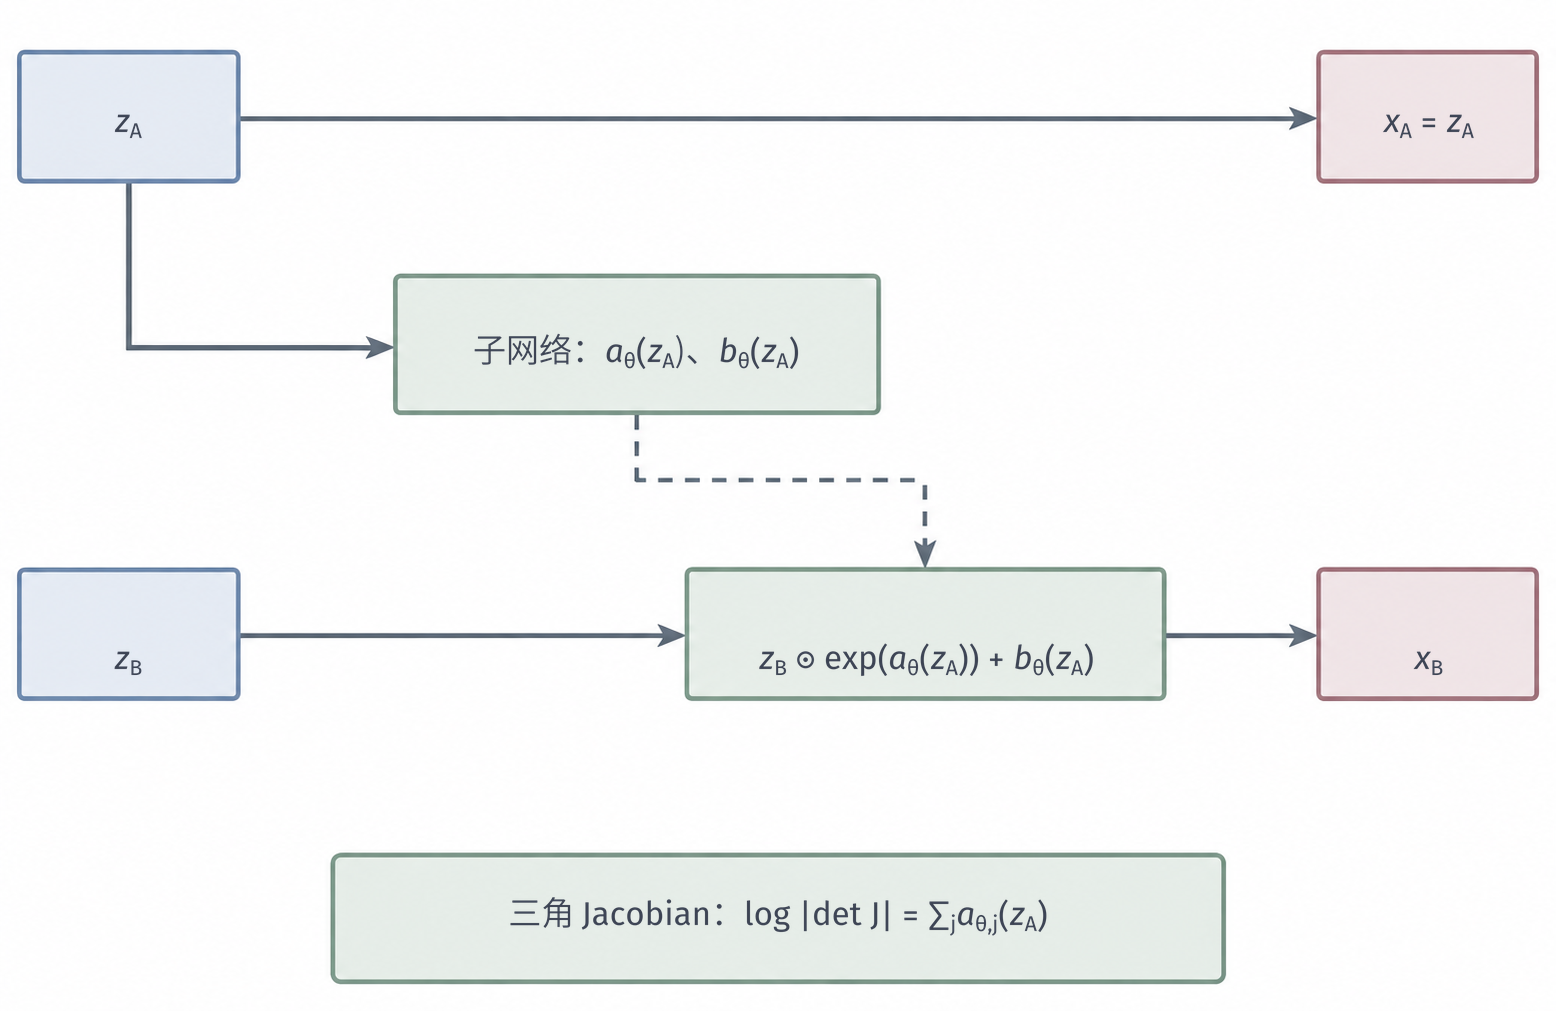
\includegraphics[width=112.000mm]{figures/03-models/03-probabilistic-graphical-models/generated/pgm-generative-coupling/figure.png}
  \caption{仿射耦合层的计算依赖。保留块$\bm z_A$经粗线进入子网络，确定$B$块仿射变换的缩放与平移。Jacobian的下三角结构使对数行列式等于缩放对数之和；逆向计算先恢复$\bm z_A$，再撤销$B$块的平移和缩放。}
  \label{fig:pgm-generative-coupling}
\end{figure}

例如，二维变换$x_1=z_1$、$x_2=2z_2+z_1^2$在$\bm{z}=(1,-1)$处输出$\bm{x}=(1,-1)$，逆变换恢复$z_2=(x_2-x_1^2)/2=-1$。Jacobian为$\left(\begin{smallmatrix}1&0\\2z_1&2\end{smallmatrix}\right)$，行列式恒为$2$。基础分布取二维标准高斯时，该观测的对数密度为$-\log(2\pi)-1-\log2$。非线性项位于Jacobian的非对角块，因此可以改变坐标依赖，同时保留简单的体积因子。

\term{自回归流}（autoregressive flow）通过坐标顺序构造三角Jacobian，用前面坐标计算当前可逆变换的参数。与直接参数化条件分布的自回归模型相比，这里需要同时考察采样方向和密度评价方向的代价（见第~\ref{chap:pgm-static-directed}章）。\term{掩码自回归流}（masked autoregressive flow, MAF）的一种形式为
\[
  x_j=\mu_j(\bm{x}_{<j})+
       \exp(a_j(\bm{x}_{<j}))z_j,\qquad j=1,\ldots,d,
\]
其中$\bm{x}_{<j}=(x_1,\ldots,x_{j-1})$。评价给定$\bm{x}$时，所有条件输入已知，掩码网络可并行给出各$\mu_j,a_j$，从而恢复$\bm{z}$并求出三角Jacobian的行列式；生成时$\bm{x}_{<j}$尚未齐备，必须顺序恢复坐标。

\term{逆自回归流}（inverse autoregressive flow, IAF）将参数输入改为$\mu_j(\bm{z}_{<j})$和$a_j(\bm{z}_{<j})$。全部基础噪声已知时，输出及对应样本密度可并行计算；给定外部观测后，逆变换则需要逐坐标恢复基础变量。因此，IAF适合生成并评价自身样本，MAF适合评价指定观测的密度，二者的顺序代价分别位于不同方向\scite{pgm-generative-papamakarios2017}

连续变换用速度场代替有限层映射。\term{连续规范化流}（continuous normalizing flow, CNF）以常微分方程
\[
  \frac{\mathrm{d}\bm{h}_u}{\mathrm{d}u}
    =\bm{v}_{\bm{\theta}}(\bm{h}_u,u),
  \qquad 0\leq u\leq1,
\]
定义基础变量到观测的映射，起点为$\bm{h}_0=\bm{z}$，终点为$\bm{h}_1=\bm{x}$，$u$表示变换进度。可逆流的一种充分正则设定是：速度场对空间连续可微，满足保证初值问题解唯一性的Lipschitz条件，且解在整个区间正反两向都存在。解的唯一性使不同轨迹在同一进度处保持分离，从而建立一一对应的变换。

记$\rho_u$为$\bm{h}_u$的密度。小步映射的Jacobian为$\bm{I}+\Delta u\,\bm{J}_{\bm{v}}+o(\Delta u)$，结合$\log\det(\bm{I}+\Delta u\,\bm{A})=\Delta u\,\operatorname{tr}\bm{A}+o(\Delta u)$，可从式~\eqref{eq:pgm-generative-flow-density}得到\term{瞬时变量变换公式}（instantaneous change of variables）：
\begin{equation}
  \label{eq:pgm-generative-instantaneous-change}
  \begin{aligned}
    \frac{\mathrm{d}}{\mathrm{d}u}
         \log\rho_u(\bm{h}_u)
       &=-\nabla_{\bm{h}}\!\cdot
          \bm{v}_{\bm{\theta}}(\bm{h}_u,u),\\
    \log p_{\bm{\theta}}(\bm{x})
       &=\log p_0(\bm{z})
         -\int_0^1\nabla_{\bm{h}}\!\cdot
           \bm{v}_{\bm{\theta}}(\bm{h}_u,u)\,\mathrm{d}u.
  \end{aligned}
\end{equation}
散度$\nabla\cdot\bm{v}=\sum_j\partial v_j/\partial h_j$为Jacobian的迹，表示局部体积膨胀率。积分该膨胀率即可追踪密度，因此CNF允许一般的速度场结构，代价转为沿轨迹反复评价速度场与散度。

高维迹计算可以采用随机估计。若随机向量满足$\mathbb{E}\bm{r}=\bm{0}$和$\mathbb{E}\bm{r}\bm{r}^{\top}=\bm{I}$，便有$\operatorname{tr}\bm{A}=\mathbb{E}_{\bm{r}}[\bm{r}^{\top}\bm{A}\bm{r}]$。自动微分通过向量与Jacobian的乘积计算单次估计，FFJORD将这一方法用于连续流\scite{pgm-generative-grathwohl2018}

该恒等式保证固定矩阵下的迹估计无偏，有限样本仍有蒙特卡洛波动。程序还需近似求解状态轨迹和散度积分，因此连续流返回的似然通常同时包含随机估计误差与数值积分误差。正向和逆向计算都依赖求解器，其成本由函数评价次数和速度场的数值性质决定。

\subsection{生成模型与变分后验}
\label{sec:pgm-generative-flow-roles}

规范化流可用于观测分布，也可用于近似后验。作为独立生成模型，它将基础变量变为观测，并由式~\eqref{eq:pgm-generative-flow-density}计算观测密度。用于VAE后验时，它在固定观测下变换简单潜变量分布，构造更灵活的$q_{\bm{\phi}}(\bm{z}\mid\bm{x})$；调整对象是推断族，生成联合分布可以保持原样\scite{pgm-overview-rezende2015}

具体地，从简单条件分布抽取$\bm{u}\sim q_0(\bm{u}\mid\bm{x})$，经$\bm{z}=f_{\bm{\phi}}(\bm{u};\bm{x})$得到后验样本。固定观测后，变换关于基础潜变量满足变量变换条件，后验样本密度便为
\begin{equation}
  \label{eq:pgm-generative-flow-posterior}
  \log q_{\bm{\phi}}(\bm{z}\mid\bm{x})
  =\log q_0(\bm{u}\mid\bm{x})
    -\log\left|
       \det\frac{\partial f_{\bm{\phi}}(\bm{u};\bm{x})}
                     {\partial\bm{u}^{\top}}
      \right|.
\end{equation}
将该密度代入$\mathbb{E}_{q_{\bm{\phi}}}[\log p_{\bm{\theta}}(\bm{x},\bm{z})-\log q_{\bm{\phi}}(\bm{z}\mid\bm{x})]$即可构造训练目标。变换后KL通常需要蒙特卡洛估计，所需联合密度和后验样本密度仍可评价。训练评价的正是本次生成的后验样本，因此可以利用IAF在这一方向上的并行计算。

扩大后验族可以收紧VAE下界，观测边缘密度仍由生成联合分布的积分定义。独立Flow则采用唯一编码$\bm{z}=f^{-1}(\bm{x})$，给定完整观测后的基础变量条件分布为点质量，两者的后验对象因此不同。

标准光滑双射也有表达限制。例如，全空间上正密度的基础分布经过处处非奇异的满射变换后，观测密度仍处处为正。这样的流可以将两个高密度区域之间的概率压低，却无法精确表示仅在两个分离区域具有支撑的密度。实现极小连接概率可能需要极端缩放，进而恶化逆变换和密度计算的数值条件。

\section{扩散与分数生成模型}
\label{sec:pgm-generative-diffusion}

\subsection{前向扰动与逆向生成}
\label{sec:pgm-generative-forward-reverse}

\term{扩散模型}（diffusion model）用逐步扰动把数据分布与简单噪声分布连接起来，并学习从噪声到数据的局部转移。训练观测提供前向加噪状态，生成则沿相反顺序执行学得的转移。下文的$\bm{x}_t$表示某一噪声尺度下的状态，索引$t$由模型人为构造；真实序列的时间索引另由动态模型描述（见第~\ref{chap:pgm-dynamic}章）。

\term{去噪扩散概率模型}（denoising diffusion probabilistic model, DDPM）的一种标准前向过程固定噪声日程$0<\beta_t<1$，$t=1,\ldots,T$，并定义
\begin{equation}
  \label{eq:pgm-generative-forward-chain}
  \begin{aligned}
    q(\bm{x}_{1:T}\mid\bm{x}_0)
      &=\prod_{t=1}^{T}q(\bm{x}_t\mid\bm{x}_{t-1}),\\
    q(\bm{x}_t\mid\bm{x}_{t-1})
      &=\mathcal{N}(\bm{x}_t;
          \sqrt{\alpha_t}\bm{x}_{t-1},\beta_t\bm{I}_d),\\
    \alpha_t&=1-\beta_t,\qquad
    \bar{\alpha}_t=\prod_{s=1}^{t}\alpha_s,\qquad
    \bar{\alpha}_0=1.
  \end{aligned}
\end{equation}
每一步缩小信号并加入独立高斯噪声。条件均值逐步乘以信号衰减系数，条件噪声方差则满足递推$\alpha_t(1-\bar{\alpha}_{t-1})+\beta_t=1-\bar{\alpha}_t$。因此，给定原观测的任意一步分布为
\begin{equation}
  \label{eq:pgm-generative-forward-marginal}
  \begin{aligned}
    q(\bm{x}_t\mid\bm{x}_0)
      &=\mathcal{N}(\bm{x}_t;
          \sqrt{\bar{\alpha}_t}\bm{x}_0,
          (1-\bar{\alpha}_t)\bm{I}_d),\\
    \bm{x}_t&=\sqrt{\bar{\alpha}_t}\bm{x}_0+
              \sqrt{1-\bar{\alpha}_t}\bm{\epsilon},
    \quad \bm{\epsilon}\sim\mathcal{N}(\bm{0},\bm{I}_d).
  \end{aligned}
\end{equation}
训练时可从该条件分布直接抽取任意噪声步，省去之前的逐步扰动计算。式中的标准高斯变量代表当前一步的合成噪声；完整前向路径的跨步依赖仍由式~\eqref{eq:pgm-generative-forward-chain}的逐步独立扰动决定。上述构造及后续目标采用DDPM的固定日程设定\scite{pgm-generative-ho2020}

有限步下，正的$\bar{\alpha}_T$使终点通常仍保留一部分数据结构。生成模型以标准高斯$p(\bm{x}_T)=\mathcal{N}(\bm{0},\bm{I}_d)$作为终端先验，日程需要使前向终点充分接近它。给定原观测时，两者的差距可以通过高斯KL直接计算：
\begin{equation}
  \label{eq:pgm-generative-terminal-kl}
  \begin{aligned}
    &\operatorname{KL}\bigl(
        q(\bm{x}_T\mid\bm{x}_0)\,\|\,p(\bm{x}_T)\bigr)\\
    &\quad=\frac12\left[
       \bar{\alpha}_T\lVert\bm{x}_0\rVert_2^2
       -d\bar{\alpha}_T-d\log(1-\bar{\alpha}_T)
      \right].
  \end{aligned}
\end{equation}
数据二阶矩有限且$\bar{\alpha}_T\to0$时，该条件KL的数据平均趋于零。KL的凸性又使这一平均量控制前向终点边缘$q_T$与先验的KL。有限步下，匹配程度取决于累计信号衰减、数据尺度和观测维度，可用该表达式评价日程选择。

在贯穿例子$X_0\sim\mathcal{N}(0,5)$中，前向边缘可以直接算出：
\begin{equation}
  \label{eq:pgm-generative-gaussian-diffusion}
  q_t(x)=\mathcal{N}(x;0,1+4\bar{\alpha}_t).
\end{equation}
取$\bar{\alpha}_T=0.25$时，终点边缘为$\mathcal{N}(0,2)$，与标准高斯的KL为$\tfrac12(2-1-\log2)\approx0.15343$。取$\bar{\alpha}_T=0.01$时，方差降至$1.04$，KL约为$0.000390$。这里评价的是终点边缘的差距；式~\eqref{eq:pgm-generative-terminal-kl}评价给定原观测的条件差距，其数据平均通常更大。

逆向生成从终端先验抽样，再逐步生成较低噪声状态：
\begin{equation}
  \label{eq:pgm-generative-reverse-joint}
  \begin{aligned}
    p_{\bm{\theta}}(\bm{x}_{0:T})
      &=p(\bm{x}_T)
          \prod_{t=1}^{T}p_{\bm{\theta}}
             (\bm{x}_{t-1}\mid\bm{x}_t),\\
    p_{\bm{\theta}}(\bm{x}_0)
      &=\int p_{\bm{\theta}}(\bm{x}_{0:T})
               \,\mathrm{d}\bm{x}_{1:T}.
  \end{aligned}
\end{equation}
终端先验和每个逆转移归一化时，联合分布及观测边缘随之归一化。中间状态作为与观测同维的潜变量，使离散扩散具有有向潜变量模型的形式。其近似推断路径由固定前向扰动核给出，因此训练可以直接构造路径样本。

\begin{figure}[htbp]
  \centering
  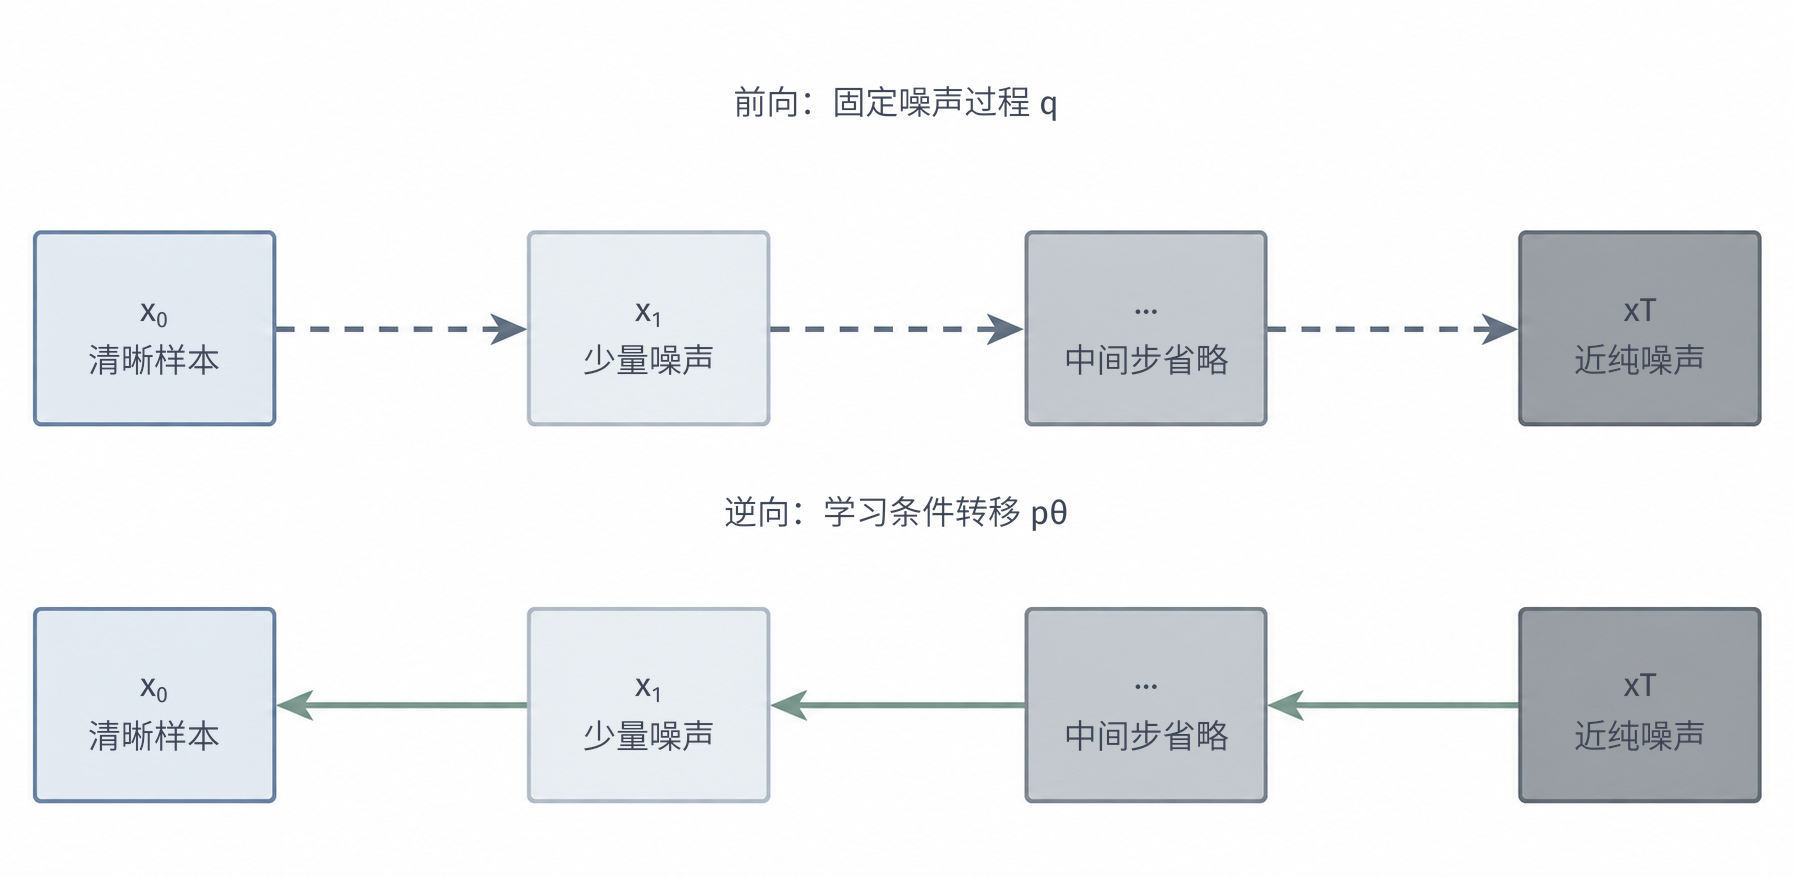
\includegraphics[width=112.000mm]{figures/03-models/03-probabilistic-graphical-models/generated/pgm-generative-diffusion/figure.png}
  \caption{离散扩散的前向扰动与逆向生成。上行按固定日程逐步加噪，下行从终端先验开始执行学得的逆转移。灰度与文字表示状态的噪声程度，相同下标对应相同噪声尺度。两行分别抽样；有限步下的终点匹配由日程和数据尺度决定。}
  \label{fig:pgm-generative-diffusion}
\end{figure}

图~\ref{fig:pgm-generative-diffusion}中的模型逆转移通常采用神经网络参数化的高斯均值与方差。真实逆转移$q(\bm{x}_{t-1}\mid\bm{x}_t)$还需对未知原观测混合，一般具有更复杂的分布形状。下面的解析高斯则额外给定原观测，描述$q(\bm{x}_{t-1}\mid\bm{x}_t,\bm{x}_0)$。因此，小步高斯是有限步模型的参数化选择，其逼近误差需要与原观测已知时的解析计算区分。

图~\ref{fig:diffusion-sample-process-illustration}通过样本插画表示噪声尺度的变化。下行以独立终端噪声启动学得的生成链，上行则由给定样本启动固定扰动链。

\begin{figure*}[htbp]
  \centering
  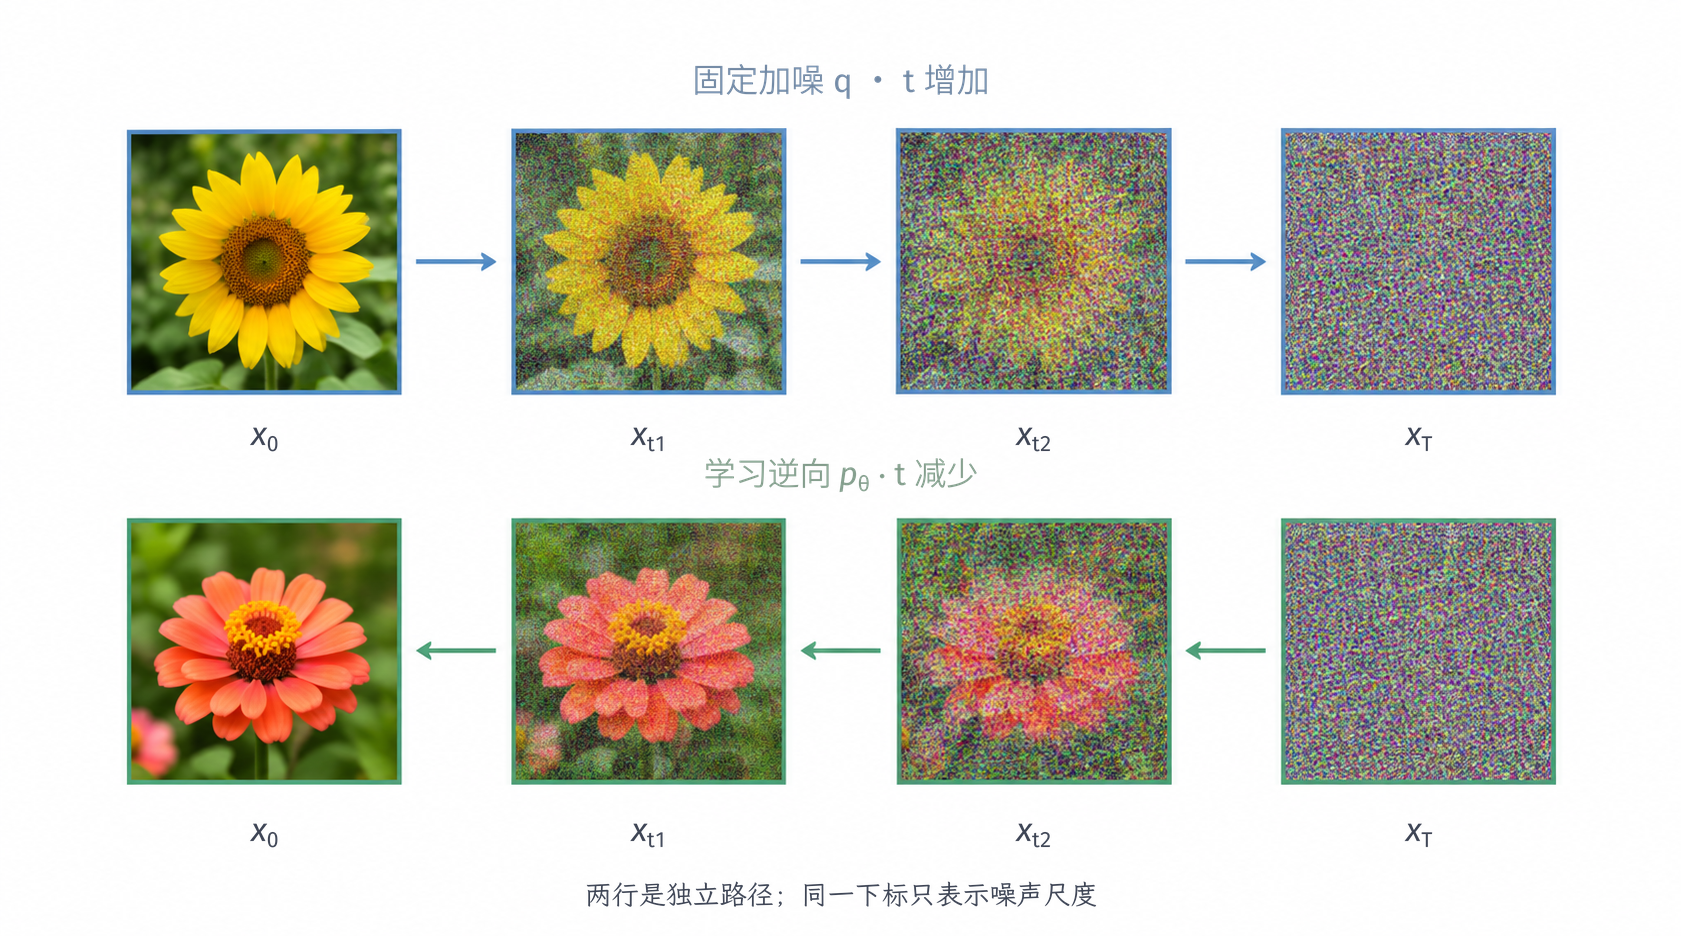
\includegraphics[width=139.534mm]{figures/03-models/03-probabilistic-graphical-models/generated/diffusion-sample-process-illustration/figure.png}
  \caption{扩散链的样本变化示意。上行从左向右逐步扰动观测，下行从右侧独立终端噪声开始向左生成；下标记录噪声尺度。花朵及中间状态为机制插画，用于说明扰动与生成方向。}
  \label{fig:diffusion-sample-process-illustration}
\end{figure*}

\subsection{变分目标与分数匹配}
\label{sec:pgm-generative-diffusion-objective}

逆向生成联合分布的学习可以采用路径变分下界。将观测固定为$\bm{x}_0$，以整条中间路径$\bm{x}_{1:T}$为潜变量，并用前向扰动分布作近似后验，一般ELBO便成为联合与前向路径密度比的期望（见式~\eqref{eq:pgm-variational-elbo}）。记路径下界为$\mathcal{B}_{\mathrm{diff}}(\bm{x}_0)$，其负值为$\mathcal{J}_{\mathrm{diff}}=-\mathcal{B}_{\mathrm{diff}}$：
\begin{equation}
  \label{eq:pgm-generative-path-elbo}
  \begin{aligned}
    \log p_{\bm{\theta}}(\bm{x}_0)
      &\geq\mathcal{B}_{\mathrm{diff}}(\bm{x}_0),\\
    \mathcal{J}_{\mathrm{diff}}(\bm{x}_0)
      &=\mathbb{E}_{q(\bm{x}_{1:T}\mid\bm{x}_0)}
         \left[\log
           \frac{q(\bm{x}_{1:T}\mid\bm{x}_0)}
                {p_{\bm{\theta}}(\bm{x}_{0:T})}
         \right].
  \end{aligned}
\end{equation}

要把这个路径比值化为局部计算，使用$t\geq2$时的Bayes恒等式
\[
  q(\bm{x}_t\mid\bm{x}_{t-1})
  =q(\bm{x}_{t-1}\mid\bm{x}_t,\bm{x}_0)
     \frac{q(\bm{x}_t\mid\bm{x}_0)}
          {q(\bm{x}_{t-1}\mid\bm{x}_0)}.
\]
将该恒等式代入前向路径密度，相邻边缘比值消去，得到同一路径密度的反向分解：
\[
  \begin{aligned}
    q(\bm{x}_{1:T}\mid\bm{x}_0)
      ={}&q(\bm{x}_T\mid\bm{x}_0)\\
         &{}\times\prod_{t=2}^{T}
              q(\bm{x}_{t-1}\mid\bm{x}_t,\bm{x}_0).
  \end{aligned}
\]
再对每个中间变量取条件期望，路径目标便分解为可局部评价的项：
\begin{equation}
  \label{eq:pgm-generative-ddpm-kl}
  \begin{aligned}
    \mathcal{J}_{\mathrm{diff}}(\bm{x}_0)
      ={}&\operatorname{KL}\bigl(
          q(\bm{x}_T\mid\bm{x}_0)\,\|\,p(\bm{x}_T)\bigr)\\
       &+\sum_{t=2}^{T}
         \mathbb{E}_{q(\bm{x}_t\mid\bm{x}_0)}
          \operatorname{KL}\bigl(
           q(\bm{x}_{t-1}\mid\bm{x}_t,\bm{x}_0)
           \,\|\,p_{\bm{\theta}}(\bm{x}_{t-1}\mid\bm{x}_t)
                         \bigr)\\
       &-\mathbb{E}_{q(\bm{x}_1\mid\bm{x}_0)}
          \log p_{\bm{\theta}}(\bm{x}_0\mid\bm{x}_1).
  \end{aligned}
\end{equation}

三部分分别评价终点匹配、逐步逆转移匹配和观测解码。固定日程与先验后，终点项与学习参数无关，求梯度时可以省略，报告完整似然界时仍计入其值。解码项评价已知观测的条件对数似然；它与中间变量的高斯KL具有不同形式，因为原观测在此已经固定。

给定原观测后，前向过程中的高斯结构使中间KL具有解析形式。对$t\geq2$，将$q(\bm{x}_t\mid\bm{x}_{t-1})q(\bm{x}_{t-1}\mid\bm{x}_0)$按待求中间变量配平方，二次项的精度系数为
\[
  \frac{\alpha_t}{\beta_t}
    +\frac{1}{1-\bar{\alpha}_{t-1}}
  =\frac{1-\bar{\alpha}_t}
          {\beta_t(1-\bar{\alpha}_{t-1})}.
\]
线性项为$\sqrt{\alpha_t}\bm{x}_t/\beta_t+\sqrt{\bar{\alpha}_{t-1}}\bm{x}_0/(1-\bar{\alpha}_{t-1})$。精度的倒数给出方差，方差与线性项相乘给出均值，因此条件分布为
\begin{equation}
  \label{eq:pgm-generative-forward-posterior}
  \begin{aligned}
    q(\bm{x}_{t-1}\mid\bm{x}_t,\bm{x}_0)
      &=\mathcal{N}(\bm{x}_{t-1};
          \widetilde{\bm{\mu}}_t,\widetilde{\beta}_t\bm{I}_d),\\
    \widetilde{\beta}_t
      &=\frac{\beta_t(1-\bar{\alpha}_{t-1})}
              {1-\bar{\alpha}_t},\\
    \widetilde{\bm{\mu}}_t
      &=\frac{\sqrt{\bar{\alpha}_{t-1}}\beta_t}
               {1-\bar{\alpha}_t}\bm{x}_0
       +\frac{\sqrt{\alpha_t}(1-\bar{\alpha}_{t-1})}
               {1-\bar{\alpha}_t}\bm{x}_t.
  \end{aligned}
\end{equation}
训练观测已知，可以直接计算这一条件均值作为监督目标。生成时只能使用当前状态、噪声步和给定外部条件，因此模型需要学习从这些输入预测相应均值。

现固定逆转移方差$\sigma_t^2>0$，令$p_{\bm{\theta}}(\bm{x}_{t-1}\mid\bm{x}_t)=\mathcal{N}(\bm{\mu}_{\bm{\theta}}(\bm{x}_t,t),\sigma_t^2\bm{I}_d)$。高斯KL分为均值误差与方差误差：
\begin{equation}
  \label{eq:pgm-generative-gaussian-step-kl}
  \begin{aligned}
    \operatorname{KL}(q\,\|\,p_{\bm{\theta}})
      &=\frac{\lVert\widetilde{\bm{\mu}}_t
                    -\bm{\mu}_{\bm{\theta}}(\bm{x}_t,t)\rVert_2^2}
               {2\sigma_t^2}+C_t,\\
    C_t&=\frac{d}{2}
       \left(\frac{\widetilde{\beta}_t}{\sigma_t^2}
              -1+\log\frac{\sigma_t^2}{\widetilde{\beta}_t}\right).
  \end{aligned}
\end{equation}
固定逆转移方差时，方差项$C_t$与待学习参数无关，常用选择为$\sigma_t^2=\beta_t$或在$t\geq2$时取$\sigma_t^2=\widetilde{\beta}_t$。逆转移方差参与学习时，均值误差权重与方差项都随参数变化，需要共同优化。若逆转移方差依赖当前状态而无待学习参数，方差项仍可在求梯度时省略，其数值则同时依赖状态与噪声步。

利用式~\eqref{eq:pgm-generative-forward-marginal}把$\bm{x}_0$换成$\bm{x}_t$和噪声，后验均值也可写成
\[
  \widetilde{\bm{\mu}}_t
  =\frac{1}{\sqrt{\alpha_t}}
       \left(\bm{x}_t-
          \frac{\beta_t}{\sqrt{1-\bar{\alpha}_t}}\bm{\epsilon}\right).
\]
该形式将均值学习转换为合成噪声预测。用网络$\bm{\epsilon}_{\bm{\theta}}(\bm{x}_t,t)$预测噪声，并据此定义模型均值：
\begin{equation}
  \label{eq:pgm-generative-noise-parameterization}
  \bm{\mu}_{\bm{\theta}}(\bm{x}_t,t)
  =\frac{1}{\sqrt{\alpha_t}}
       \left(\bm{x}_t-
          \frac{\beta_t}{\sqrt{1-\bar{\alpha}_t}}
               \bm{\epsilon}_{\bm{\theta}}(\bm{x}_t,t)\right).
\end{equation}
回到仅随噪声步变化的固定逆转移方差设定，两均值相减时$\bm{x}_t$项抵消。记$\ell_t(\bm{\theta})$为第$t$个中间KL的数据与扰动平均，并仍按式~\eqref{eq:pgm-generative-forward-marginal}抽取$\bm{x}_t$，则
\begin{equation}
  \label{eq:pgm-generative-weighted-denoising}
  \begin{aligned}
    \ell_t(\bm{\theta})
      &=w_t\,\mathbb{E}_{\bm{x}_0,\bm{\epsilon}}
         \lVert\bm{\epsilon}
          -\bm{\epsilon}_{\bm{\theta}}(\bm{x}_t,t)\rVert_2^2+C_t,\\
    w_t&=\frac{\beta_t^2}
              {2\sigma_t^2\alpha_t(1-\bar{\alpha}_t)},
          \qquad t=2,\ldots,T.
  \end{aligned}
\end{equation}
这一权重由固定逆转移方差下的高斯KL推导而来，通常随噪声步变化，因此决定不同噪声尺度对ELBO学习的相对贡献。

\begin{example}[核对一个扩散步的权重]
  \label{ex:pgm-generative-step-weight}
  取便于手算的噪声系数$\beta_1=0.2$、$\beta_2=0.25$，于是$\alpha_2=0.75$、$\bar{\alpha}_1=0.8$、$\bar{\alpha}_2=0.6$。在$t=2$时，给定原观测的条件方差为$\widetilde{\beta}_2=0.25(0.2)/0.4=0.125$。若模型逆转移方差取$\sigma_2^2=0.25$，去噪权重为$w_2=0.25^2/(2\cdot0.25\cdot0.75\cdot0.4)=5/12$。一维噪声预测误差取$0.3$，对应均值差的平方为
  \[
    \frac{0.25^2}{0.75\cdot0.4}(0.3)^2=0.01875,
  \]
  除以$2\sigma_2^2=0.5$得到$0.0375$，与$(5/12)(0.3)^2$一致。再加方差项$C_2=\tfrac12(0.5-1+\log2)\approx0.09657$，便得到完整KL。本例用较大的噪声系数核对均值参数化与去噪权重的代数关系。
\end{example}

DDPM还常用均匀抽步的噪声平方回归作为简化目标。独立抽取$t\sim\operatorname{Unif}\{1,\ldots,T\}$、$\bm{x}_0\sim p_{\mathrm{data}}$和$\bm{\epsilon}\sim\mathcal{N}(\bm{0},\bm{I}_d)$，定义
\begin{equation}
  \label{eq:pgm-generative-simple-loss}
  \mathcal{J}_{\mathrm{simple}}
  =\mathbb{E}_{t,\bm{x}_0,\bm{\epsilon}}
      \lVert\bm{\epsilon}
       -\bm{\epsilon}_{\bm{\theta}}(\bm{x}_t,t)\rVert_2^2.
\end{equation}
该目标为所有噪声步采用相同回归权重，并在$t=1$继续预测噪声。它改变了原ELBO中各尺度的权衡，报告似然下界时需回到完整路径目标。原始DDPM对离散像素以量化区间积分定义解码质量；连续数据采用固定方差高斯解码时，解码负对数似然则包含特定权重的平方误差及常数项。因此，简化噪声损失与这些解码项、逐步加权KL的数值不同\scite{pgm-generative-ho2020}

严格ELBO也可以通过随机抽步优化。对中间步按正概率$\pi_t$抽取$t\in\{2,\ldots,T\}$，用$w_t\lVert\bm{\epsilon}-\bm{\epsilon}_{\bm{\theta}}\rVert_2^2/\pi_t$无偏估计其中依赖参数的求和，并单独计算解码项。均匀抽步时，校正因子为中间步数；报告完整界值还需计入方差常数和终点项。

抽步概率的改变配合重要性校正，可以调整估计方差而保留原目标。直接改变步权重则调整训练准则。若模型表达能力不受限、各尺度可独立拟合，任意正权重都保留逐尺度平方回归的最优条件均值；有限共享网络需在不同尺度间分配容量，权重因而影响实际拟合结果。

噪声回归还可以理解为密度梯度学习。记前向扰动后的边缘密度为$q_t(\bm{x})$，其\term{分数}（score）$\bm{s}_t^*(\bm{x})=\nabla_{\bm{x}}\log q_t(\bm{x})$给出对数密度局部增加的方向。本章用$q_t$与前向路径记号保持一致，分数模型文献也常将该边缘记为$p_t$。虽然边缘分数未知，高斯扰动的条件分数可以直接计算：
\[
  \nabla_{\bm{x}_t}\log q(\bm{x}_t\mid\bm{x}_0)
  =-\frac{\bm{x}_t-\sqrt{\bar{\alpha}_t}\bm{x}_0}
           {1-\bar{\alpha}_t}
  =-\frac{\bm{\epsilon}}{\sqrt{1-\bar{\alpha}_t}}.
\]
若可以交换微分与积分，对$q_t(\bm{x}_t)=\int q(\bm{x}_t\mid\bm{x}_0)p_{\mathrm{data}}(\bm{x}_0)\,\mathrm{d}\bm{x}_0$求导并除以$q_t(\bm{x}_t)>0$，得到
\begin{equation}
  \label{eq:pgm-generative-denoising-identity}
  \bm{s}_t^*(\bm{x}_t)
  =\mathbb{E}\!\left[
       \nabla_{\bm{x}_t}\log q(\bm{x}_t\mid\bm{X}_0)
       \mid\bm{x}_t\right]
  =-\frac{\mathbb{E}[\bm{\epsilon}\mid\bm{x}_t]}
            {\sqrt{1-\bar{\alpha}_t}}.
\end{equation}
平方回归的总体最优预测为条件均值。因此，令$\bm{s}_{\bm{\theta}}=-\bm{\epsilon}_{\bm{\theta}}/\sqrt{1-\bar{\alpha}_t}$，噪声预测对应各尺度边缘分数的估计。给定受扰动状态后，多种原观测与噪声都可能产生它，回归目标中的随机噪声通过条件平均形成可预测部分。

\term{去噪分数匹配}（denoising score matching, DSM）以已知扰动核的条件分数训练未知边缘分数。令$\bm{a}=\nabla_{\bm{x}_t}\log q(\bm{x}_t\mid\bm{X}_0)$；在平方矩有限时，条件期望的正交分解把训练误差写为
\begin{equation}
  \label{eq:pgm-generative-dsm-decomposition}
  \mathbb{E}\lVert\bm{s}_{\bm{\theta}}-\bm{a}\rVert_2^2
  =\mathbb{E}\lVert\bm{s}_{\bm{\theta}}-\bm{s}_t^*\rVert_2^2
   +\mathbb{E}\lVert\bm{a}-\bm{s}_t^*\rVert_2^2.
\end{equation}
最后一项与网络参数无关，因此最小化条件分数误差等价于最小化边缘分数误差。对当前高斯核，噪声平方误差为条件分数平方误差乘以$(1-\bar{\alpha}_t)$。简化噪声损失与严格ELBO因而对应不同的DSM尺度加权，只有从指定生成模型推导的权重及其余项才组成该模型的ELBO。连续时间分数建模将这些噪声尺度连接起来\scite{pgm-generative-song2021}

把式~\eqref{eq:pgm-generative-noise-parameterization}改用分数表示，还得到
\[
  \bm{\mu}_{\bm{\theta}}(\bm{x}_t,t)
    =\frac{\bm{x}_t+\beta_t\bm{s}_{\bm{\theta}}(\bm{x}_t,t)}
            {\sqrt{\alpha_t}}.
\]
使用真分数时，该式给出真实逆转移的条件均值；转移的完整形状仍由数据分布决定。式~\eqref{eq:pgm-generative-gaussian-diffusion}的一维例子给出真分数$-x_t/(1+4\bar{\alpha}_t)$，代入即可核对均值。

分数也联系能量模型：若$q_t(\bm{x})\propto\exp[-E_t(\bm{x})]$，则$\bm{s}_t^*=-\nabla E_t$，因为归一化常数对空间求导后消失（见第~\ref{chap:pgm-energy-models}章）。一般向量网络近似分数时，还需额外条件才能把它表示为标量能量的梯度；直接评价归一化密度也需要相应密度构造。

算法~\ref{alg:pgm-generative-ddpm}采用连续观测，逆转移方差均预先固定且为正。全部转移均值由噪声网络按式~\eqref{eq:pgm-generative-noise-parameterization}计算，包括$t=1$的高斯解码分布$p_{\bm{\theta}}(\bm{x}_0\mid\bm{x}_1)$。同一噪声损失因而训练各步均值，解码阶段使用这组共享参数。

\begin{algorithm}[固定方差DDPM的学习与祖先采样]
  \label{alg:pgm-generative-ddpm}
  \begin{algorithmic}[1]
    \Require 连续观测数据集、固定$\beta_{1:T}$及正的逆转移方差$\sigma_{1:T}^2$
    \Ensure 学得的噪声网络与模型样本
    \State 初始化$\bm{\theta}$，预计算$\alpha_t,\bar{\alpha}_t$
    \For{每个训练小批量，直至停止条件满足}
      \State 为每个观测抽$t\sim\operatorname{Unif}\{1,\ldots,T\}$和标准高斯$\bm{\epsilon}$
      \State 按式~\eqref{eq:pgm-generative-forward-marginal}计算$\bm{x}_t$
      \State 由式~\eqref{eq:pgm-generative-simple-loss}更新参数
    \EndFor
    \State 抽$\bm{x}_T\sim\mathcal{N}(\bm{0},\bm{I}_d)$
    \For{$t=T,T-1,\ldots,2$}
      \State 用噪声网络和式~\eqref{eq:pgm-generative-noise-parameterization}计算$\bm{\mu}_{\bm{\theta}}$
      \State 独立抽$\bm{\xi}_t\sim\mathcal{N}(\bm{0},\bm{I}_d)$，令$\bm{x}_{t-1}=\bm{\mu}_{\bm{\theta}}+\sigma_t\bm{\xi}_t$
    \EndFor
    \State 抽$\bm{x}_0\sim p_{\bm{\theta}}(\bm{x}_0\mid\bm{x}_1)$并返回
  \end{algorithmic}
\end{algorithm}

算法采用简化训练损失。严格变分学习可将训练步骤替换为带权中间项估计和解码负对数似然。连续高斯解码的末步方差需单独指定正值，因为解析前向后验的$\widetilde{\beta}_1=0$对应已固定的原观测。末步也可以约定输出预测均值，但这种输出省去了正方差解码分布的随机波动。

设一次网络前向代价为$C_{\mathrm{net}}$，随机抽步训练的单样本前向代价约为$O(C_{\mathrm{net}}+d)$，完整祖先采样则为$O(T(C_{\mathrm{net}}+d))$。采样只需保留当前状态；评价全路径变分界还需处理全部项，或采用带校正的随机估计。训练抽步的计算收益因此与多步生成的成本并存。

\subsection{连续时间表示与采样}
\label{sec:pgm-generative-continuous-diffusion}

细化噪声步后，可以用连续索引$t\in[0,T_{\mathrm{c}}]$描述扰动，$T_{\mathrm{c}}$为终点。本节采用扩散系数仅依赖时间的各向同性设定，使逆向公式具有明确的分数项。设$\bm{W}_t$为$d$维标准\term{布朗运动}（Brownian motion），其不相交区间增量相互独立，长度$\Delta t$的增量服从$\mathcal{N}(\bm{0},\Delta t\,\bm{I}_d)$。前向\term{随机微分方程}（stochastic differential equation, SDE）为
\begin{equation}
  \label{eq:pgm-generative-forward-sde}
  \mathrm{d}\bm{X}_t
  =\bm{b}(\bm{X}_t,t)\,\mathrm{d}t
    +g(t)\,\mathrm{d}\bm{W}_t,
  \qquad \bm{X}_0\sim p_{\mathrm{data}}.
\end{equation}
漂移$\bm{b}$规定确定性的局部移动，$g(t)>0$规定噪声强度。为保证前向解存在且不爆炸，假设系数连续，漂移对空间全局Lipschitz且至多线性增长，噪声系数有界并在所讨论闭区间上有正下界。

使用反向密度公式还需密度和逆过程的正则性：假设$q_t>0$，对时间一阶、对空间二阶连续可微，所用时间区间上$\int\mathbb{E}_{q_t}\lVert\nabla\log q_t(\bm{X}_t)\rVert_2^2\,\mathrm{d}t<\infty$，且反向方程存在不爆炸的解。数据分布本身奇异时，可将这些条件限定于$t\geq\delta>0$的已加噪区间，观测端点另行处理。

与离散DDPM相应的方差保持过程采用$\bm{b}(\bm{x},t)=-\tfrac12\beta(t)\bm{x}$和$g(t)=\sqrt{\beta(t)}$。条件均值的衰减系数为$\exp[-\tfrac12\int_0^t\beta(s)\,\mathrm{d}s]$，条件方差为$1-\exp[-\int_0^t\beta(s)\,\mathrm{d}s]$。有限终点内的累计噪声积分有限时，仍有一部分原信号保留；终点与标准高斯的匹配需要通过累计扰动强度控制。

条件扰动核可解析时，可以从连续区间抽取噪声尺度，构造受扰动观测，再拟合条件分数$\nabla_{\bm{x}_t}\log q(\bm{x}_t\mid\bm{x}_0)$。式~\eqref{eq:pgm-generative-denoising-identity}和式~\eqref{eq:pgm-generative-dsm-decomposition}在满足条件的每个正噪声尺度上继续说明其边缘分数含义。时间抽样密度与损失权重共同决定训练比重；观测似然评价则需要后文的密度构造与积分计算。

记真分数为$\bm{s}_t^*=\nabla_{\bm{x}}\log q_t$。在上述正则条件及反向过程存在的设定下，反向SDE可以沿同一个$t$写成
\begin{equation}
  \label{eq:pgm-generative-reverse-sde}
  \begin{aligned}
    \mathrm{d}\bm{X}_t
    ={}&\bigl[\bm{b}(\bm{X}_t,t)-g(t)^2\bm{s}_t^*(\bm{X}_t)\bigr]
         \,\mathrm{d}t\\
       &+g(t)\,\mathrm{d}\overline{\bm{W}}_t,
    \qquad t:T_{\mathrm{c}}\downarrow0.
  \end{aligned}
\end{equation}
该式沿递减时间积分，$\mathrm{d}t<0$，反向布朗增量的协方差为$|\mathrm{d}t|\bm{I}_d$。实现时可改用递增反向索引$u=T_{\mathrm{c}}-t$，令$\bm{Y}_u=\bm{X}_{T_{\mathrm{c}}-u}$，将时间方向显式写入漂移：
\begin{equation}
  \label{eq:pgm-generative-positive-reverse-time}
  \begin{aligned}
    \mathrm{d}\bm{Y}_u
      ={}&-\bm{b}(\bm{Y}_u,T_{\mathrm{c}}-u)\,\mathrm{d}u\\
         &+g(T_{\mathrm{c}}-u)^2
              \bm{s}_{T_{\mathrm{c}}-u}^*(\bm{Y}_u)\,\mathrm{d}u\\
         &+g(T_{\mathrm{c}}-u)\,\mathrm{d}\bm{B}_u.
  \end{aligned}
\end{equation}
其中$\bm{B}_u$为递增反向索引下的标准布朗运动。该路径反演结果使用真分数及上述正则条件，其证明依赖随机过程反演理论。分数SDE框架还讨论了状态相关扩散系数；相应逆漂移包含扩散矩阵的空间导数，需采用更一般的公式\scite{pgm-generative-song2021}

式~\eqref{eq:pgm-generative-positive-reverse-time}也给出明确的数值一步。令$t=T_{\mathrm{c}}-u$、$\Delta u>0$，用学得分数替代真分数的Euler--Maruyama更新为
\[
  \begin{aligned}
    \bm{y}_{u+\Delta u}
      ={}&\bm{y}_u-\bm{b}(\bm{y}_u,t)\Delta u\\
         &+g(t)^2\bm{s}_{\bm{\theta}}(\bm{y}_u,t)\Delta u
          +g(t)\sqrt{\Delta u}\,\bm{\xi},
  \end{aligned}
\]
每一步独立抽取$\bm{\xi}\sim\mathcal{N}(\bm{0},\bm{I}_d)$。递增反向索引下，分数项为正号，真分数使该部分漂移沿对数密度增加方向移动；式~\eqref{eq:pgm-generative-reverse-sde}则将相同方向放在负时间增量中。精确恢复前向数据分布需要真实终点分布、真分数和精确求解。实际生成中的终端先验近似、分数估计和离散积分分别产生不同误差。

真分数可得时，还可以用确定性流保持前向SDE的各时刻边缘密度。\term{概率流常微分方程}（probability flow ordinary differential equation, probability flow ODE）采用速度场
\begin{equation}
  \label{eq:pgm-generative-probability-flow}
  \frac{\mathrm{d}\bm{X}_t}{\mathrm{d}t}
     =\bm{v}^*(\bm{X}_t,t),
  \qquad
  \bm{v}^*(\bm{x},t)
     =\bm{b}(\bm{x},t)-\frac12g(t)^2\bm{s}_t^*(\bm{x}).
\end{equation}
概率流速度中的分数系数为逆SDE对应系数的一半。给定终点后，ODE轨迹由速度场确定，样本之间的随机性来自终点抽样。下面通过密度守恒说明这一系数。

前向SDE的Fokker--Planck方程描述边缘密度随时间的变化：
\[
  \partial_t q_t
    =-\nabla\cdot(\bm{b}q_t)+\tfrac12g(t)^2\Delta q_t.
\]
利用$q_t\bm{s}_t^*=\nabla q_t$以及$g$不依赖$\bm{x}$，右侧等于
\[
  -\nabla\cdot
       \left[\left(\bm{b}-\tfrac12g(t)^2\bm{s}_t^*\right)q_t\right],
\]
该表达式是速度场$\bm{v}^*$的连续性方程。在适当边界衰减、共同初始密度及密度方程唯一性条件下，两种过程因此具有相同的单时刻边缘。路径分布仍不同：SDE包含沿途随机增量，ODE在给定初始点后采用确定性轨迹。

使用学得分数时，令$\bm{v}_{\bm{\theta}}=\bm{b}-\tfrac12g^2\bm{s}_{\bm{\theta}}$，并指定可评价密度的终端先验$p_{T_{\mathrm{c}}}$。速度场若生成正反两向均存在的可微流，终端分布及逆流便定义ODE密度模型$p_{\bm{\theta}}^{\mathrm{ODE}}$。沿数据到终点的轨迹积分瞬时变量变换公式，可评价这个模型的密度：
\begin{equation}
  \label{eq:pgm-generative-ode-likelihood}
  \begin{aligned}
    \log p_{\bm{\theta}}^{\mathrm{ODE}}(\bm{x}_0)
       &=\log p_{T_{\mathrm{c}}}(\bm{x}_{T_{\mathrm{c}}})
          +\int_0^{T_{\mathrm{c}}}
            \nabla_{\bm{x}}\cdot
            \bm{v}_{\bm{\theta}}(\bm{x}_t,t)\,\mathrm{d}t,\\
    \frac{\mathrm{d}\bm{x}_t}{\mathrm{d}t}
       &=\bm{v}_{\bm{\theta}}(\bm{x}_t,t),
       \qquad \bm{x}_{t=0}=\bm{x}_0.
  \end{aligned}
\end{equation}
瞬时公式表示终点对数密度减去起点对数密度等于负散度积分。移项求起点密度后，式中的散度积分因此取正号。密度评价从数据积分到终点，生成则从终端先验反向积分；两者采用同一速度场。

例如一维速度$v(x,t)=ax$、$T_{\mathrm{c}}=1$、终端密度$\mathcal{N}(0,1)$时，$x_1=e^a x_0$，散度积分为$a$，所以
\[
  \log p^{\mathrm{ODE}}(x_0)
  =-\tfrac12\log(2\pi)-\tfrac12e^{2a}x_0^2+a.
\]
结果等于$\mathcal{N}(0,e^{-2a})$的对数密度。取$a=-\tfrac12\log5$即得到$\mathcal{N}(0,5)$，其中散度积分提供正确的归一化因子。该线性场例子用于核对ODE变量变换的积分方向，速度场由本例单独指定。

式~\eqref{eq:pgm-generative-ode-likelihood}评价的是指定速度场与终端先验所定义的ODE分布。使用近似分数时，同一网络驱动的随机SDE通常定义另一分布，有限步DDPM又由其离散转移定义边缘。因此，三者的似然比较需要先确定模型对象；同边缘结果适用于真分数、匹配终点和精确求解的设定。

密度数值评价沿轨迹计算散度。随机迹估计产生蒙特卡洛误差，有限容差求解器产生轨迹与积分误差，两项计算相互耦合；固定矩阵上的无偏迹估计只处理其中一项性质。减小求解器容差和增加迹样本分别针对数值积分与随机估计，分数偏差和终点失配仍需通过模型学习与日程选择处理。

若把观测端点截断到$\delta>0$，所评价的是截断模型在该噪声尺度的密度，观测空间的概率还需通过后续解码或近似确定。离散像素似然另涉及量化区间质量或去量化下界，比较时需统一预处理及测度。

采样成本可以用网络函数评价次数衡量：高阶ODE步骤可能调用网络多次，自适应求解器还可能拒绝试步。随机采样沿途引入噪声，确定性采样在固定终点后便于重复生成与编码；两者的质量需在相同网络、预算和评价准则下比较。减少数值步通常降低计算，同时改变离散化误差。对有限步DDPM，完整执行全部转移对应该离散模型的祖先采样，跳过转移则需另行评价近似误差。

\term{采样蒸馏}（sampling distillation）进一步用一个已训练采样器的多步输出监督另一个少步模型。渐进蒸馏可把两个确定性教师步骤压成一个学生步骤，重复这一过程降低生成时的函数评价次数\scite{pgm-generative-salimans2022}

蒸馏将部分生成计算转移到额外训练，并引入学生对教师映射的近似。学生若需要评价密度，还需给出自身的密度构造与求值机制；采用可逆映射时，可以通过相应的体积变化追踪密度。扩散索引始终表示人为噪声尺度；用于视频等真实时序数据时，可对整个序列或其潜表示加噪，真实时间与噪声尺度各自承担不同的索引角色。

\section{模型关系与比较}
\label{sec:pgm-generative-comparison}

\subsection{似然、后验与采样}
\label{sec:pgm-generative-likelihood-posterior-sampling}

完整观测密度、部分观测下的条件分布、潜变量后验和无条件样本，构成四种不同查询。Flow可直接评价完整密度，部分观测查询仍可能需要边缘积分；VAE编码器快速给出近似后验，其误差由后验族、共享映射和优化决定；DDPM训练可以随机抽步，祖先生成则按逆转移顺序执行。固定查询对象后，模型的计算优势才能直接比较。

\term{概率电路}（probabilistic circuit, PC）通过计算图的结构约束支持概率查询。叶节点表示可精确评价和边缘化的简单分布，和节点执行加权混合，乘积节点组合不同变量块。查询沿图中的加法与乘法传播，为完整密度和边缘概率提供另一种计算安排\scite{pgm-generative-choi2020}

一种充分设定是将归一化的叶分布逐层组合，并令和节点的权重非负且和为$1$。和节点的各个孩子涉及同一组变量，这一条件称为\term{光滑性}（smoothness），也称完备性。乘积节点的各个孩子涉及互不相交的变量组，这一条件称为\term{可分解性}（decomposability）。从叶向根归纳，加权和保持归一化，不相交变量块上的乘积也保持归一化。边缘化时，先在叶节点积分，再沿原图进行加法与乘法传播；可分解性使不同变量块的积分能够拆开。设电路边数为$m$、叶查询代价为常数，一次向上传播的代价为$O(m)$。条件化分母的边缘概率质量或密度为正时，条件分布由两个相应边缘量之比得到。

线性传播成本相对于给定电路大小而言；复杂分布可能需要很大的表示。MAP和边缘MAP包含最大化，对混合分量的求和与最大化如何交换另需结构条件，因此其计算要求与边缘概率不同。概率电路由此说明，支持完整密度评价和支持大量边缘查询需要不同的结构安排。表~\ref{tab:pgm-generative-model-comparison}按查询对象概括各机制。

\begin{table*}[htbp]
  \centering
  \small
  \begin{tabularx}{\linewidth}{@{}lXXX@{}}
    \toprule
    机制 & 完整观测的似然 & 潜变量与条件查询 & 典型采样代价与限制 \\
    \midrule
    自回归基线
      & 条件分解给出精确似然
      & 一般缺失坐标不一定能高效边缘化
      & 通常按坐标顺序生成；依赖排序 \\
    VAE
      & 通常优化ELBO，边缘似然需额外估计
      & 编码器给出近似后验
      & 先抽潜变量再解码；条件似然决定额外成本 \\
    离散层Flow
      & 逆变换与Jacobian可行时精确
      & 完整观测有唯一逆像；部分观测仍可能需积分
      & 逐层变换；自回归流有方向性成本 \\
    DDPM
      & 路径ELBO可估计；简化损失不是似然值
      & 固定前向路径充当变分分布
      & 多步随机转移；有限终点与参数化有误差 \\
    分数ODE
      & 散度积分定义ODE模型密度
      & 可逆流给出编码，不是随机路径后验
      & 数值积分；精度与函数评价次数相关 \\
    受约束概率电路
      & 可精确评价归一化密度或质量
      & 合适结构下可精确边缘化与条件查询
      & 结构化采样；表示规模可能很大 \\
    \bottomrule
  \end{tabularx}
  \caption{不同生成机制的查询与采样成本。“精确”表示相应模型的数学计算关系可以直接评价，实际实现仍有浮点误差；连续流和分数ODE另需数值积分，并可能使用随机迹估计。概率电路采用正文的光滑性、可分解性及归一化条件。}
  \label{tab:pgm-generative-model-comparison}
\end{table*}

似然比较需要相同观测表示、测度和预处理。样本中的任务结构、模式覆盖和生成成本则由相应指标分别评价。一维例子中的三种机制都可表达$\mathcal{N}(0,5)$，潜变量关系与生成路径却不同；仅凭观测边缘无法识别这些内部机制。

在表达能力方面，VAE的生成族、Flow的可逆结构和扩散的逆转移族分别限制候选分布。增加网络容量可以改善函数拟合，但Flow的支撑约束、VAE的条件似然假设及有限步高斯逆转移的形状限制仍取决于模型结构。

在收敛性方面，需要先确定优化目标：VAE优化下界，离散Flow直接优化似然，扩散可优化路径下界或尺度加权的去噪目标。非凸参数化、随机梯度、近似推断和数值求解分别影响能否达到目标最优值，以及所需迭代和每次迭代成本；下界变紧或回归误差下降本身只回答相应训练目标的改进。

在泛化性方面，训练找到的候选分布还需在未参与拟合的观测上评价。样本量与模式覆盖、候选族容量、参数约束和训练终止共同影响这种表现，数据采集分布的改变还会改变预测任务。留出似然或其明确的估计、任务样本质量和模式覆盖应分别报告；网络训练的收敛与泛化分析可参考第~\ref{chap:neural-network-training}章和第~\ref{chap:neural-network-generalization}章。

\subsection{生成机制的组合}
\label{sec:pgm-generative-hybrids}

组合生成机制时，先确定被调整的概率对象。采用Flow后验扩大$q_{\bm{\phi}}(\bm{z}\mid\bm{x})$的表达范围，主要针对近似族误差。新族包含原族时，理论最优下界至少与原来相同，实际改善仍取决于优化。采用Flow先验则改变$p_{\bm{\theta}}(\bm{z})$，调整无条件生成时访问潜空间的方式。同类可逆网络因此可以承担推断和生成两种不同角色。

层次VAE通过多个随机潜变量层表示观测依赖。对于前文的两层例子，若取$q_{\bm{\phi}}(\bm{z}_1,\bm{z}_2\mid\bm{x})=q_{\bm{\phi}}(\bm{z}_1\mid\bm{x})q_{\bm{\phi}}(\bm{z}_2\mid\bm{z}_1,\bm{x})$，ELBO就是
\[
  \mathbb{E}_{q_{\bm{\phi}}}
  \left[
    \log\frac{
      p(\bm{z}_2)p_{\bm{\theta}}(\bm{z}_1\mid\bm{z}_2)
          p_{\bm{\theta}}(\bm{x}\mid\bm{z}_1)}
      {q_{\bm{\phi}}(\bm{z}_1\mid\bm{x})
          q_{\bm{\phi}}(\bm{z}_2\mid\bm{z}_1,\bm{x})}
  \right].
\]
下界继续采用生成联合与变分路径密度比的期望，可通过逐层抽样估计。每层后验都需与相应生成依赖匹配，层次模型因而仍存在推断误差和潜变量利用问题。扩散的多层潜状态还配有噪声尺度、固定前向核及专门的局部目标，这些安排决定了它与一般层次VAE的计算差异。

\term{潜空间扩散}（latent diffusion）把多步生成放在观测的潜表示中：先学习编码与解码，再在编码得到的潜变量分布上训练扩散模型，最后把生成的潜变量解码为观测。其主要计算收益来自反复去噪的空间更小；原始潜空间扩散工作在预训练自编码表示上构造这一过程\scite{pgm-generative-rombach2022}

若解码器是归一化条件分布$p_{\bm{\psi}}(\bm{x}\mid\bm{z})$，潜空间生成先验为$p_{\bm{\theta}}^{\mathrm{diff}}(\bm{z})$，整体模型为
\begin{equation}
  \label{eq:pgm-generative-latent-diffusion}
  p_{\bm{\theta},\bm{\psi}}(\bm{x})
  =\int p_{\bm{\psi}}(\bm{x}\mid\bm{z})
          p_{\bm{\theta}}^{\mathrm{diff}}(\bm{z})\,\mathrm{d}\bm{z}.
\end{equation}
整体观测密度仍由潜变量积分给出，其计算包含潜空间生成和条件解码两部分。非可逆确定性解码器或主要由感知损失训练的编码过程，需要另行规定观测空间的概率语义，才能评价像素似然。压缩造成的信息损失、潜空间分布的拟合误差和解码族限制分别作用于生成结果；组合收益需连同这些代价一起评价。

\subsection{与隐式生成模型的边界}
\label{sec:pgm-generative-implicit-boundary}

假设只给出$\bm{Z}\sim p_0$和生成程序$\bm{X}=G_{\bm{\theta}}(\bm{Z})$。对任意可测集合$B$，它已经规定
\begin{equation}
  \label{eq:pgm-generative-pushforward}
  \mathbb{P}_{\bm{\theta}}(\bm{X}\in B)
  =\int \mathbf{1}\{G_{\bm{\theta}}(\bm{z})\in B\}
           p_0(\bm{z})\,\mathrm{d}\bm{z}.
\end{equation}
这种通过采样程序间接规定的分布称为\term{隐式分布}（implicit distribution）。\term{生成对抗网络}（generative adversarial network, GAN）是常见例子：通常的生成器提供样本，却不提供像式~\eqref{eq:pgm-generative-flow-density}那样可直接评价的观测密度。这里将GAN作为通过生成程序定义分布的例子，相关比较针对密度与采样查询\scite{pgm-generative-goodfellow2014}

密度评价涉及逆像计算，也涉及采用的测度。同维光滑映射即使处处局部可逆，全局多对一时通常仍需累加所有逆像的贡献，普通网络未必支持枚举这些逆像。若基础变量维度低于观测维度，局部Lipschitz生成网络的输出还可能集中于低维集合，在整个观测空间的Lebesgue测度下没有密度。推送公式依然定义合法分布，相应查询需要采用适合该分布的概率表达。

Flow同样将噪声推送为观测，并进一步利用同维可逆变换和可计算体积因子评价密度。VAE与离散扩散则给出可评价的联合分布，把观测密度明确写为潜变量边缘积分，进而构造似然下界。生成程序、密度存在性、密度求值算法和下界估计因此对应不同性质；模型提供哪些查询，可由这些具体概率构造判断。

\section{本章小结}
\label{sec:pgm-generative-summary}

概率生成模型通过不同结构协调归一化、密度评价、推断和采样。VAE用潜变量边缘化定义观测密度，以近似后验和ELBO学习参数；规范化流为完整观测建立唯一逆像，用Jacobian追踪局部体积；扩散以人工噪声过程构造潜状态，通过局部去噪目标学习逆向生成。三种机制可以组合，也可以表达相同观测分布，其潜变量含义和查询成本仍各有差异。

训练目标由具体概率构造决定。VAE重构项来自观测似然，后验灵活性影响下界差距；DDPM路径ELBO由终点项、逐步加权KL和解码项组成，均匀噪声回归调整了尺度权衡。连续逆SDE需结合积分方向解释漂移符号，概率流ODE的同边缘结果使用真分数及匹配边界。ODE模型的密度评价另需散度积分，其实现同时受数值求解和随机迹估计影响。

选择模型时，所需查询确定评价重点：潜变量推断关注后验误差，完整密度评价关注逆变换或边缘积分，缺失变量查询关注边缘化结构，低延迟生成关注网络评价次数与顺序依赖。进一步分析表达能力、收敛性和泛化性，可以分别判断候选分布的限制、训练达到目标的条件与成本，以及新观测上的表现。样本质量与这些概率查询各自提供证据，共同说明模型在具体任务中的作用。

\paragraph{扩展阅读}
VAE原论文介绍近似后验与变分下界，Rezende与Mohamed讨论用可逆变换扩展变分后验，Sohl-Dickstein等介绍逐步噪声的生成过程。三项工作分别适合进一步考察后验近似、推断族表达能力和多步随机生成；阅读时可将密度求值与采样成本对应到各自的概率构造\scite{kingma2013,pgm-overview-rezende2015,pgm-overview-sohl2015}
